% thesis_takada.tex
% ##################################################
\documentclass[a4paper,12pt]{article_vdlab_sotsuron}
\pagestyle{plain}

\usepackage{setspace}
\usepackage{graphicx}
\usepackage{amsmath,amssymb}
\usepackage{colortbl}
\usepackage{comment}
\usepackage{multirow}

\begin{document}
%文字間隔を設定
\kanjiskip = .0pt plus 3pt minus 3pt
\xkanjiskip = .0pt plus 3pt minus 3pt
\small
\setstretch{1.5}

% ##################################################
\begin{center}
  % 論文題目
  \jtitle{HILSシステムにおける\\アクチュエータの制御手法の検討}
  \etitle{Study on Actuator Control Method with\\ Hardware-in-the-Loop Simulation System}
\end{center}

%目次の表示
\tableofcontents

\newpage
\section{序論}
\subsection{タイヤとサスペンション}
タイヤは自動車において唯一路面と接触する要素であり,自動車の基本的な機能である「走る」「曲がる」「止まる」といった運動は,すべて路面とタイヤとの間に発生する摩擦力によって実現している\cite{1}.そのため,タイヤは車両運動特性に大きな影響を与える重要な要素といえる.したがって,タイヤの特性を十分理解することで車両の運動特性を把握し,その性能を十分に発揮させることができる\cite{2}.また,車体とタイヤはサスペンションによって連結されている.サスペンションは,車体重量を支持すると共に,車輪の上下振動を緩和,吸収して,振動が車体に直接伝達されることを防止する.また,路面間に発生する駆動力,制動力,横力など各種の路面反力を車体に伝達することで,車両運動性能に影響を与える.したがって,車両運動特性を把握するためには,タイヤとサスペンションを複合的に評価する必要がある.図~\ref{fig:tire_suspention}~にタイヤ-サスペンション機構を示す.

\vspace*{10mm}
\begin{figure}[h]
  \begin{center}
    \includegraphics[height=70mm]{figure/tire_suspension.eps}
    \vspace*{3mm}
    \caption{Tire-Suspension\cite{3}}
    \label{fig:tire_suspention}
  \end{center}
\end{figure}

% **************************************************
\newpage
\subsection{Hardware-in-the-Loop Simulation(HILS)システム}
車両運動性能を評価する手法として,シミュレーションや実車走行試験などが挙げられる.しかし,シミュレーションでは,評価対象のモデル化誤差が生じ,実車走行試験では,同一条件での試験が困難である.このような問題を解決するシステムとしてHILSシステムが用いられている\cite{4}.HILSとは,Hardware-in-the-Loop Simulationの略であり,ハードウェアの計測結果を用いたリアルタイム解析によりアクチュエータを制御することによって、特性評価を行う手法である.このHILSシステムは,従来の時刻歴シミュレーションと実機試験のそれぞれの欠点を補完するのようなものとなり,シミュレーション精度の向上を図りながら,試験に必要なコストを抑え,試験の自由度を確保することができる.このため,部品開発の一段階としてHILS試験を導入することで,精度と効率の両面において質の高い試験が可能となり,開発の大幅な効率化が期待できる.\cite{5}.

\vspace*{10mm}
\begin{figure}[htp]
  \begin{center}
    \includegraphics[height=50mm]{figure/HILS_system.eps}
    \vspace*{3mm}
    \caption{HILS System\cite{6}}
    \label{fig:HILS_system}
  \end{center}
\end{figure}

\subsection{研究目的}
前述のようにHILSシステムはハードウェアの計測結果を含む解析モデルの計算結果に基づいてアクチュエータの入力を決定し特性評価を行うシステムである.
\par
そこで本研究では,自動車のタイヤ-サスペンション系の上下動をHILSシステムを用いて評価を行う。アクチュエータの制御手法として,路面-車体間の相対変位を用いる手法と,試験機の特性を同定した結果を用いる手法について検討し評価試験を実施し,試験の挙動と解析結果を比較することでそれぞれの制御手法におけるHILSシステムの再現性を評価した.また,試験機のサスペンション部に摩擦を生じさせ、その影響を評価関数を用いてリアルタイムに評価し,路面-車体間の相対変位を用いる手法において考慮し評価試験を実施し,アクチュエータの制御手法がHILSシステムに及ぼす影響を評価した.


% #################################################
\newpage
\section{HILSシステムの構成}
\subsection{ハードウェア}
\subsubsection{HILS試験機}本研究で開発したHILS試験機を図~\ref{HILSmachine}に示す.
この装置は上下1自由度で路面部にアクチュエータを取り付けている.
自動車の車体をばね上で,タイヤ-サスペンション系をばね下とばね・ダンパで表現している.
\par
ソフトウェア部で計算したサスペンションストロークをばね上ばね下間の変位として実現している.
また,レーザ変位計とロードセルを用いて,サスペンションストロークとダンパ力を計測している.

%  ーーーーーーーーーーーーーーーーーーーーーーーーーーーーーーー
% Tire testing machine
%  ーーーーーーーーーーーーーーーーーーーーーーーーーーーーーーー
\vspace{24mm}
\begin{figure}[h]
  \begin{center}
  \includegraphics[height=80mm]{figure/HILS_machine_T.eps}
  \vspace{4mm}
   \caption{HILS Testing Machine}
  \label{HILSmachine}
  \end{center}
\end{figure}

\newpage
\subsubsection{摩擦を付与する機構}
本研究室ではHILSシステムにおける摩擦の影響を確認するために図~\ref{friction_hard}に示すような機構を取り付けた.この機構は六角支柱,ブラケット,ウレタンゴム,アルミフレームによって構成されている.ウレタンゴムの硬度はショアA32である.六角支柱はステンレスナットによって固定されている.またCAD図を図~\ref{friction_cad}に示す.

\vspace{10mm}
\begin{figure}[h]
  \begin{center}
  \includegraphics[height=60mm]{figure/friction_hard.eps}
  \vspace{4mm}
   \caption{Mechanism to give friction}
  \label{friction_hard}
  \end{center}
\end{figure}

\vspace{10mm}
\begin{figure}[h]
  \begin{center}
  \includegraphics[height=60mm]{figure/friction_cad.eps}
  \vspace{4mm}
   \caption{Mechanism to give friction(CAD)}
  \label{friction_cad}
  \end{center}
\end{figure}

\newpage
\subsubsection{ばねの選定}
本研究室で開発された試験機のばねには錆が生じていた.また,ばねにサージング現象がみられたため,路面入力試験機を行ったときに意図していない振動が発生してしまう.図~\ref{fig:spring_pri}~は選定する前のHILS試験機に6mmのステップ入力を行ったときのサスペンションストロークである.ステップ入力直後に高周波な振動が現れていることがわかる.この現象を軽減するために路面入力試験を行う前にばねを選定した.選定する条件として5.5kgの荷重を加えたとき,取り付け位置が150mm程度になり,さらに30mmの圧縮が可能である条件とした.選定する前と選定したばねの外観を図~\ref{fig:spring_pri}~,図~\ref{fig:spring_new}~に示す.選定したばねの諸元を\ref{tab:spring}に示す.ばねの選定は株式会社アキュレイトの選ばね君を参考に行った\cite{spring_order}.選定した結果,ばねのサージング現象は抑えることができたが,HILS試験機に振幅1mmのような小さな入力を行ったときに$m_1$部が動かなくなってしまうことが起こってしまった.

\vspace{5mm}
\begin{figure}[h]
  \begin{center}
  \includegraphics[height=35mm]{figure/1_close_step_6.eps}
  \vspace{4mm}
   \caption{Suspension stroke(Ordered spring)}
  \label{surging}
  \end{center}
\end{figure}

\begin{figure}[h!]
  \begin{tabular}{cc}
  \begin{minipage}{0.5\hsize}
  \begin{center}
    \includegraphics[height=40mm]{figure/spring_pri.eps}
      \vspace*{3mm}
      \caption{Ordered Spring(SWP-B)}
      \label{fig:spring_pri}
    \end{center}
  \end{minipage}
  \begin{minipage}{0.5\hsize}
     \begin{center}
      \includegraphics[height=40mm]{figure/spring_new.eps}
      \vspace*{3mm}
      \caption{OrderSpring(SUS-316-WPA)}
      \label{fig:spring_new}
    \end{center}
  \end{minipage}
  \end{tabular}
 \end{figure}

  \begin{table}[h!]
    \begin{center}
      \makeatletter
      \def\@captype{table}
      \makeatother
      \caption{Specification of Oder Spring}
        \label{tab:spring}
  	\begin{tabular}{cc}\hline
  	  Parameter & Value\\\hline
  	  Material & SUS316-WPA\\
  	  Wire Diameter  & 4.0[mm]\\
  	  OuterDiamenter & 90[mm]\\
  	  Number of Active Coils & 8[-]\\
  	  Free Length & 280[mm]\\
      Spring constant & 0.439[N/mm]\\\hline
        \end{tabular}
      \end{center}
  \end{table}
\newpage
\subsubsection{アクチュエータ}
ここでは,アクチュエータとして用いるモータとその制御ユニットとして用いるモータドライバについて説明する.
\par
まず,本試験機に用いるモータはmaxon japan株式会社のECモータ「EC-max 40 283867」である.モータの外観を図~\ref{fig:ecmax40}~に,モータスペックを表~\ref{tab:ecmax40}~に示す.モータの先端にはギアヘッドが取り付けられ,回転方向や角度を検出する電子部品としてエンコーダが取り付けられている.このモータにはmaxon japan株式会社のプラネタリギアヘッド「GP42C 203126」とエンコーダ「HEDL5540 110516」を取り付けた.そでぞれの仕様を表~\ref{tab:113:1}~,表~\ref{tab:500pulse}~に示す.

\vspace*{10mm}
\begin{figure}[htp]
  \begin{minipage}{0.4\textwidth}
    \begin{center}
      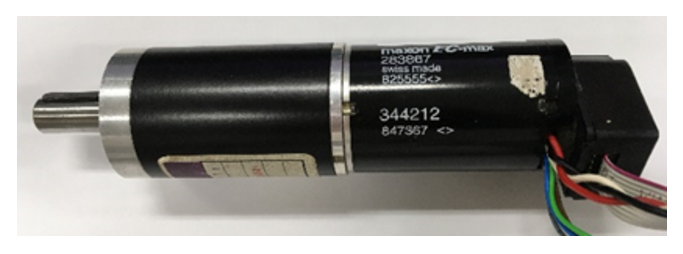
\includegraphics[height=20mm]{figure/ecmax40.eps}
      \vspace*{3mm}
      \caption{ECmax40 283867}
      \label{fig:ecmax40}
    \end{center}
  \end{minipage}
  \begin{minipage}{0.6\textwidth}
      \begin{center}
	\makeatletter
	\def\@captype{table}
	\makeatother
	\caption{Specification of EC Servomotor(283867)}
	\label{tab:ecmax40}
	  \begin{tabular}{cc}\hline
	    Nominal output & 70 [W] \\
	    Nominal voltage & 24 [V] \\
	    Nominal speed & 12000 [rpm] \\
	    Max continuous Torque & 89.6 [mNm] \\
	    Max continuous current & 3.44 [A] \\
	    Torque constant & 28 [mNm/A] \\
	    Speed constant & 341 [rpm/V] \\\hline
	  \end{tabular}
	\end{center}
  \end{minipage}
\end{figure}

\vspace*{10mm}
\begin{table}[htp]
  \begin{minipage}{0.5\textwidth}
    \begin{center}
      \makeatletter
	\def\@captype{table}
	\makeatother
	\caption{Specification Gearhead(203126)}
	\label{tab:113:1}
	  \begin{tabular}{cc}\hline
	    Gear Ratio & 113:1 \\
	    Rated speed & 8000 [rpm] \\
	    Backlash & 1.0 [deg] \\
	    Max continuous torque & 15 [Nm] \\\hline
	  \end{tabular}
    \end{center}
  \end{minipage}
  \begin{minipage}{0.5\textwidth}
      \begin{center}
	\makeatletter
	\def\@captype{table}
	\makeatother
	\caption{Specification of Encoder(110516)}
	\label{tab:500pulse}
	  \begin{tabular}{cc}\hline
	    Encoder Resolution & 500 [count/rev] \\
	    Max frequency & 100 [kHz] \\
	    Allowable maximum speed & 12000 [rpm] \\\hline
	  \end{tabular}
	\end{center}
  \end{minipage}
\end{table}
\newpage
\subsubsection{モータドライバ}
次に,モータドライバについて説明する.先ほどのモータの制御ユニットとして,maxon japan株式会社の「EPOS2 70/10 375711」を使用した.モータドライバの外観を図~\ref{fig:epos}~に,仕様を表~\ref{tab:epos}~に示す.EPOS2は,インクリメンタル・エンコーダ付きDCモータおよびEC(ブラシレス)モータを駆動可能なデジタル位置制御ユニットである.CANopen,USB 2.3/3.0,RS232通信による通信を可能とし,Point to Pointの位置制御,回転数制御,トルク制御を行うことができる.EPOS2 70/10は,モジュール式のデジタル位置制御ユニットで,80~700Wまでのエンコーダ付きDCモータ,またはホールセンサ/エンコーダ付きブラシレスECモータに対応している.本研究では,RS232通信を用いて位置指令を行い,「Position Mode」を用いた位置制御によりモータを制御している.電源電圧の供給には,図~\ref{fig:rs_150_24}~に示すMEAN WELL社のスイッチング電源「RS-150-24」を使用した.

\vspace*{10mm}
\begin{figure}[htp]
  \begin{minipage}{0.4\textwidth}
    \begin{center}
      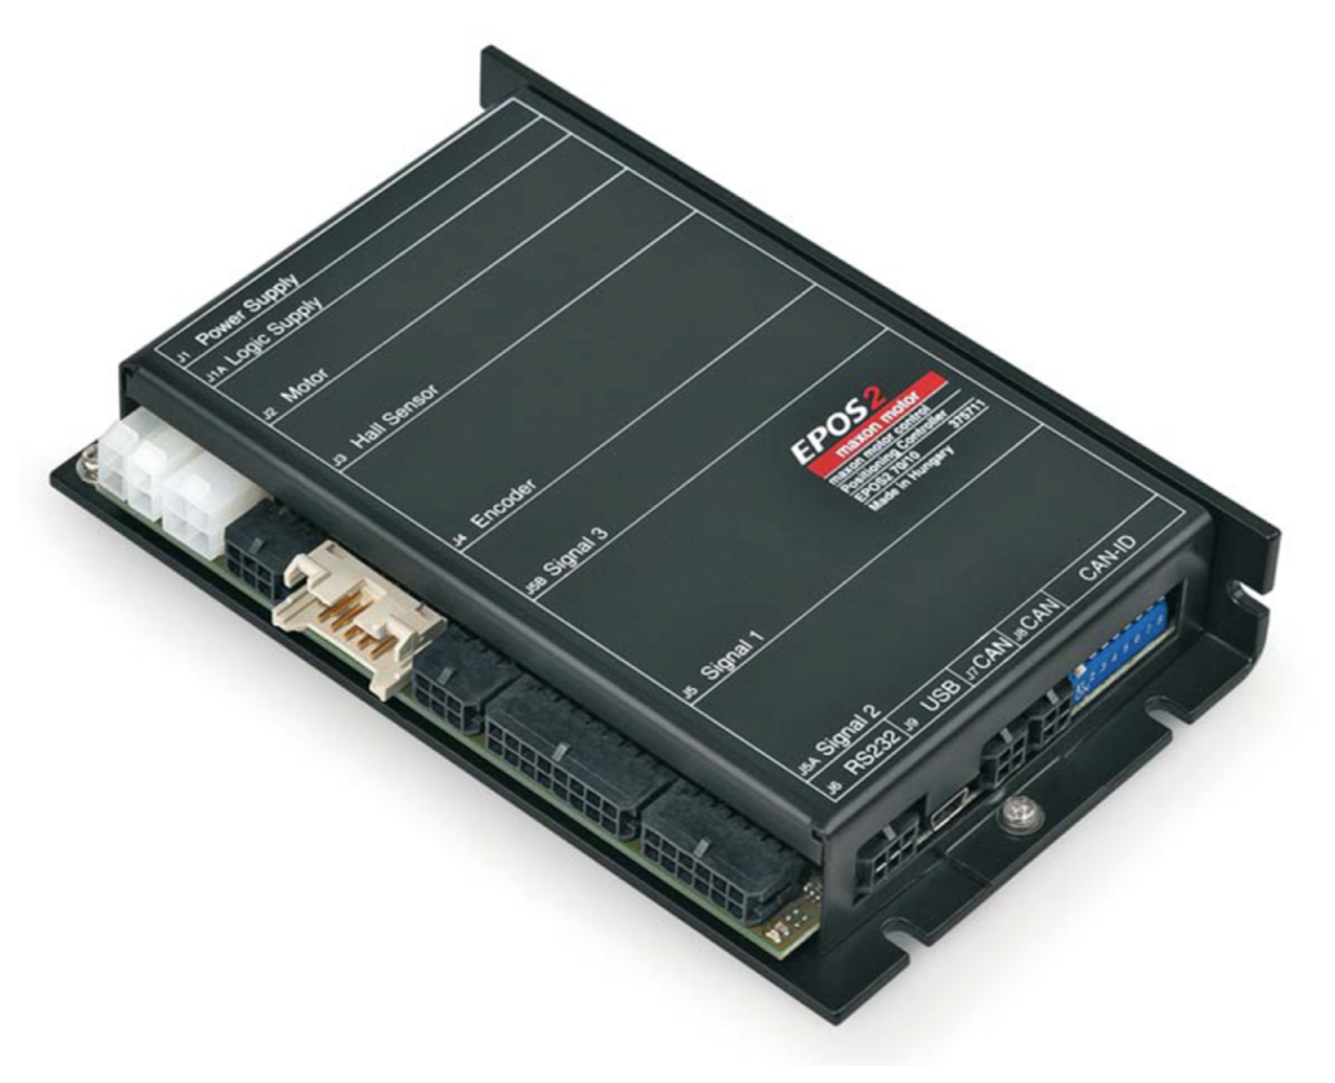
\includegraphics[height=40mm]{figure/epos.eps}
      \vspace*{3mm}
      \caption{EPOS2 70/10(375711)}
    \label{fig:epos}
    \end{center}
  \end{minipage}
  \begin{minipage}{0.6\textwidth}
      \begin{center}
	\makeatletter
	\def\@captype{table}
	\makeatother
	\caption{Specification of EPOS2 70/10(375711)}
	\label{tab:epos}
	\begin{tabular}{cc}\hline
	  power suppy voltage [VDC] & 11-70\\
	  Max output current [A] & 25\\
	  Max continuous current [A] & 10\\
	  Hall sensor & H1, H2, H3 \\
	  Encoder & A, A$\setminus$, B, B$\setminus$, I, I$\setminus$(max. 5MHz)\\
	  Analog Input & 2(differential, 12-bit, 0...+5 V)\\
	  RS232 & RxD; TxD(max. 115200 bit/2) \\\hline
	  \end{tabular}
	\end{center}
  \end{minipage}
\end{figure}

\vspace*{10mm}
\begin{figure}[htp]
  \begin{center}
    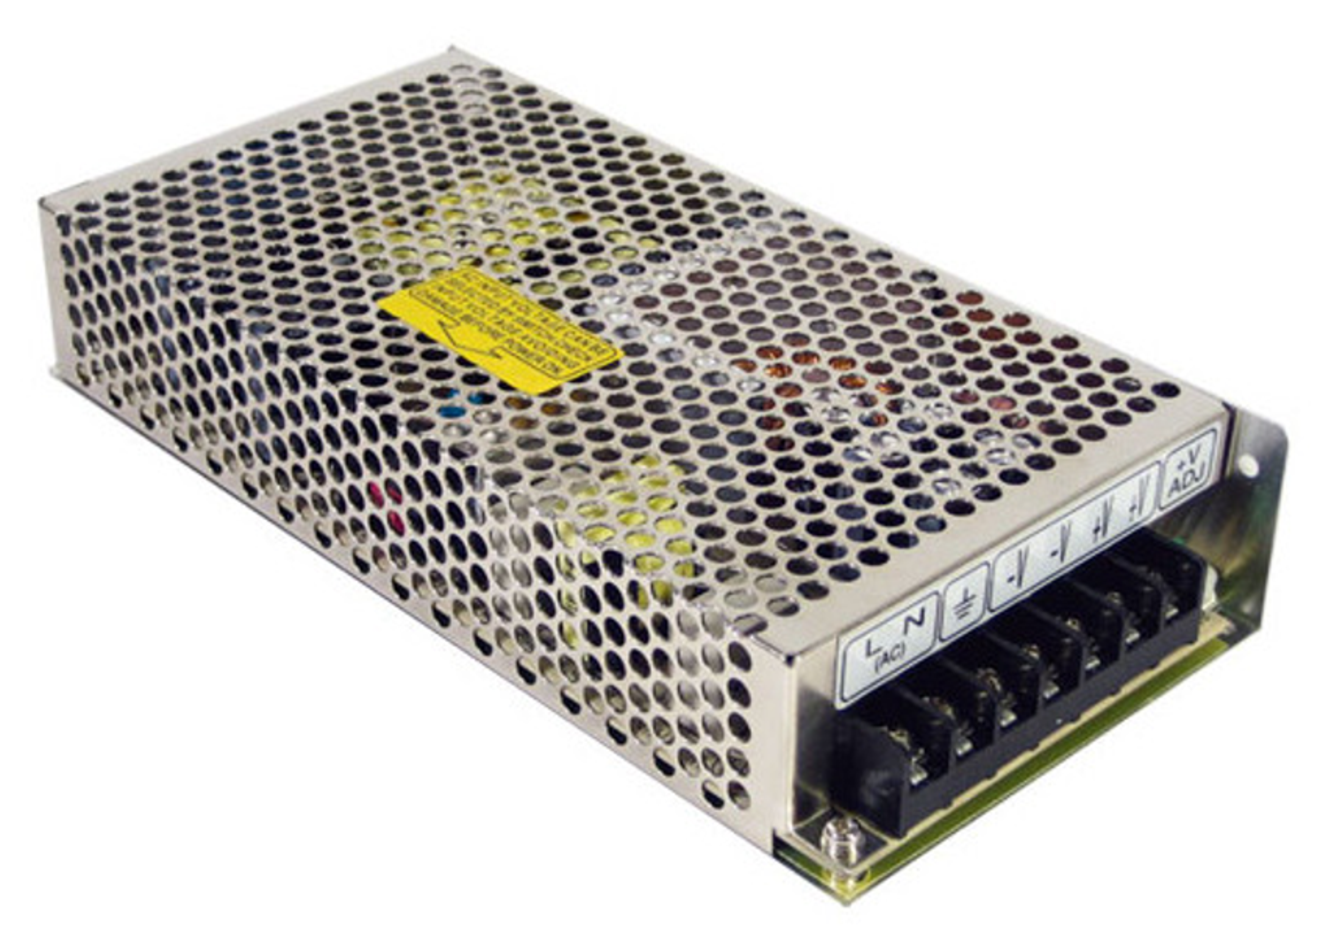
\includegraphics[height=40mm]{figure/rs_150_24.eps}
    \vspace*{3mm}
    \caption{Swiching Power Supply(RS-150-24)}
    \label{fig:rs_150_24}
  \end{center}
\end{figure}

\newpage
本研究では、シリアル通信を用いて位置制御を行った。それにあたり、RS232ケーブルを用いてPC-PC間でシリアル通信を用いて値を送り、モータドライバの使用方法を確認した。送信に使用したSimulinkを図~\ref{fig:serial_send}~、受信に使用したSimulinkを図~\ref{fig:serial_recieve}~に示す。通信周期は2msで行った。シリアル通信を行う際、表~\ref{tab:serial}~に示すような設定が必要であり、Simulinkの「Serial Configration」ブロックを用いて設定した。図~\ref{fig:serial_send}~にある「MATLAB Function」ブロックは付録に示す。これは、ETH Zurich(スイス連邦工科大学チューリッヒ校)のAutonomous Systems Laboratoryが公開しているGitHub(ethz-asl/matlab-epos-librery)を参考にした。\cite{99}

\vspace*{10mm}
\begin{figure}[htp]
  \begin{center}
    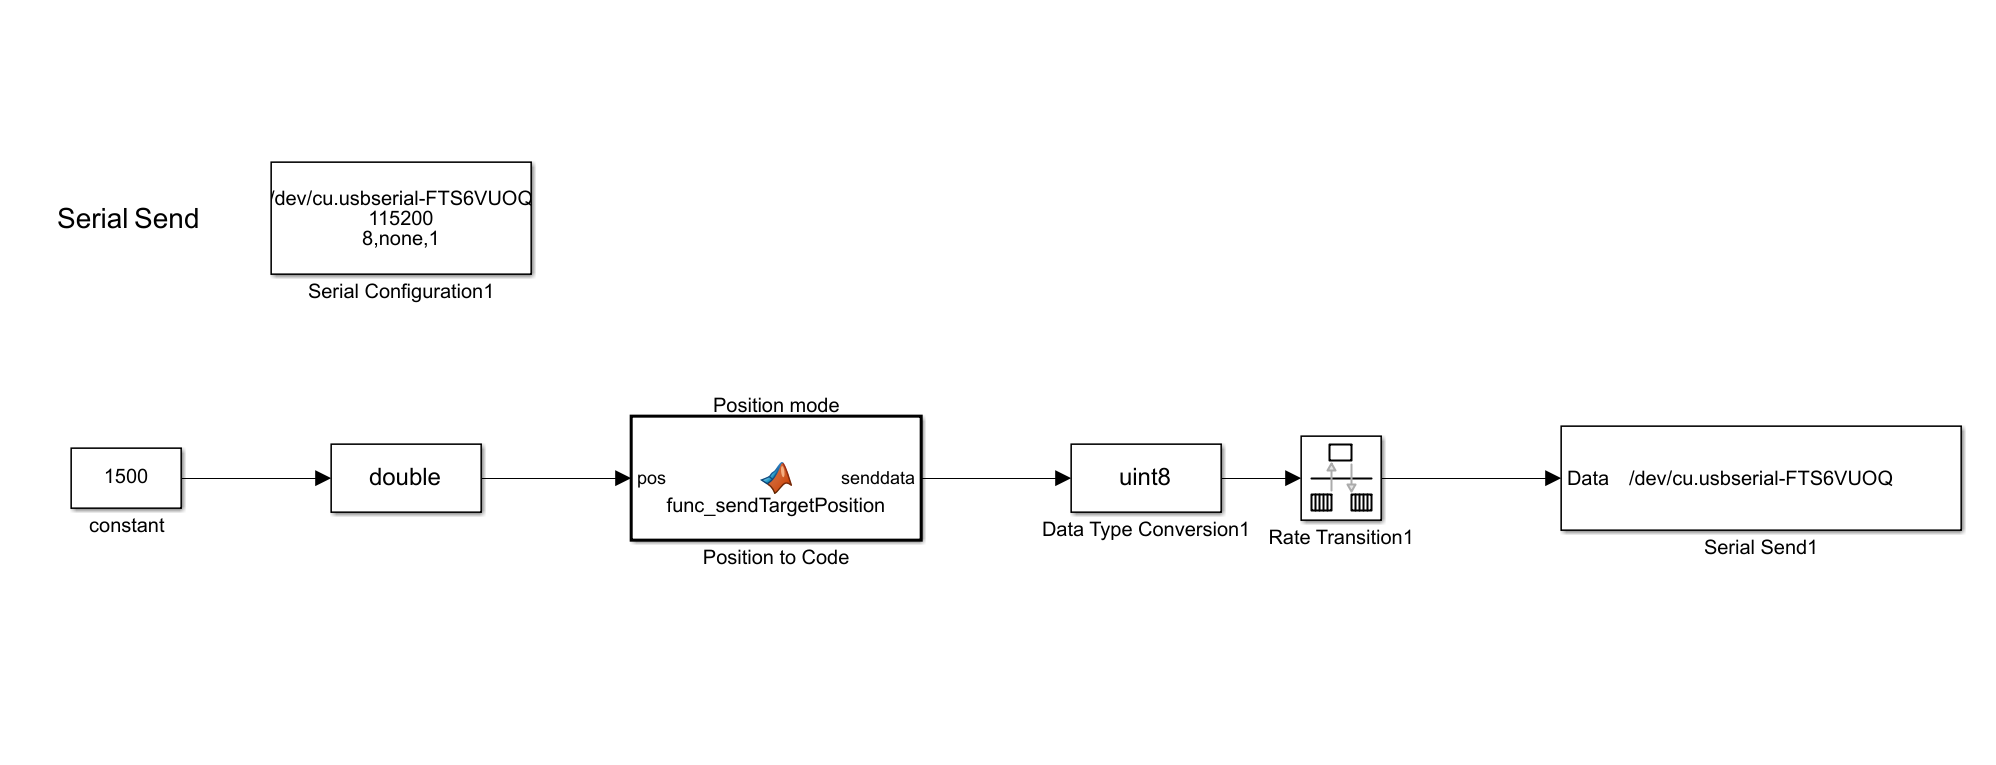
\includegraphics[height=40mm]{figure/serial_send.eps}
    \vspace*{3mm}
    \caption{Serial Send}
    \label{fig:serial_send}
  \end{center}
\end{figure}

\vspace*{10mm}
\begin{figure}[htp]
  \begin{center}
    \includegraphics[height=60mm]{figure/serial_recieve.eps}
      \vspace*{3mm}
      \caption{Serial Recieve}
      \label{fig:serial_recieve}
  \end{center}
\end{figure}

\newpage
\begin{table}[htp]
  \begin{center}
    \makeatletter
    \def\@captype{table}
    \makeatother
    \caption{Specification of Serial Communication(RS232)}
      \label{tab:serial}
	\begin{tabular}{cc}\hline
	  Parameter & Value\\\hline
	  Baud Rate & 115200 [bps]\\
	  Start Bits & 1\\
	  Data Bits & 8\\
	  Parity & none\\
	  Stop Bits & 1\\
	  Byte Order & Little Endian\\
	  Terminator & $\backslash$n\\\hline
      \end{tabular}
    \end{center}
\end{table}

\vspace*{10mm}
このモータドライバと路面部モータであるECブラシレスモータ「EC22 386658」を用いて位置制御の確認を行った。モータドライバ「EPOS2 70/10 375711」はmaxon motor社製のグラフィカル・ユーザ・インターフェース「EPOS Studio」を用いて、モータやエンコーダなどにモータドライバが適合するようにシステム設定を行うことができる。\cite{22}また、制御ゲインのオート・チューニング機能を用いて、電流、速度、位置の制御ゲインを自動的に調整している。図~\ref{fig:serial_send}~の送信先をモーダドライバに設定した。オシロスコープを使って通信が正常に行われていることと、モータが動作することを確認した。なお、オシロスコープでは通信周期の2msごとに0Vと1Vに切り替わる矩形波を見ることができる。図~\ref{fig:epos_studio}~に「EPOS Studio」の画面を示す。

\vspace*{10mm}
\begin{figure}[htp]
  \begin{center}
    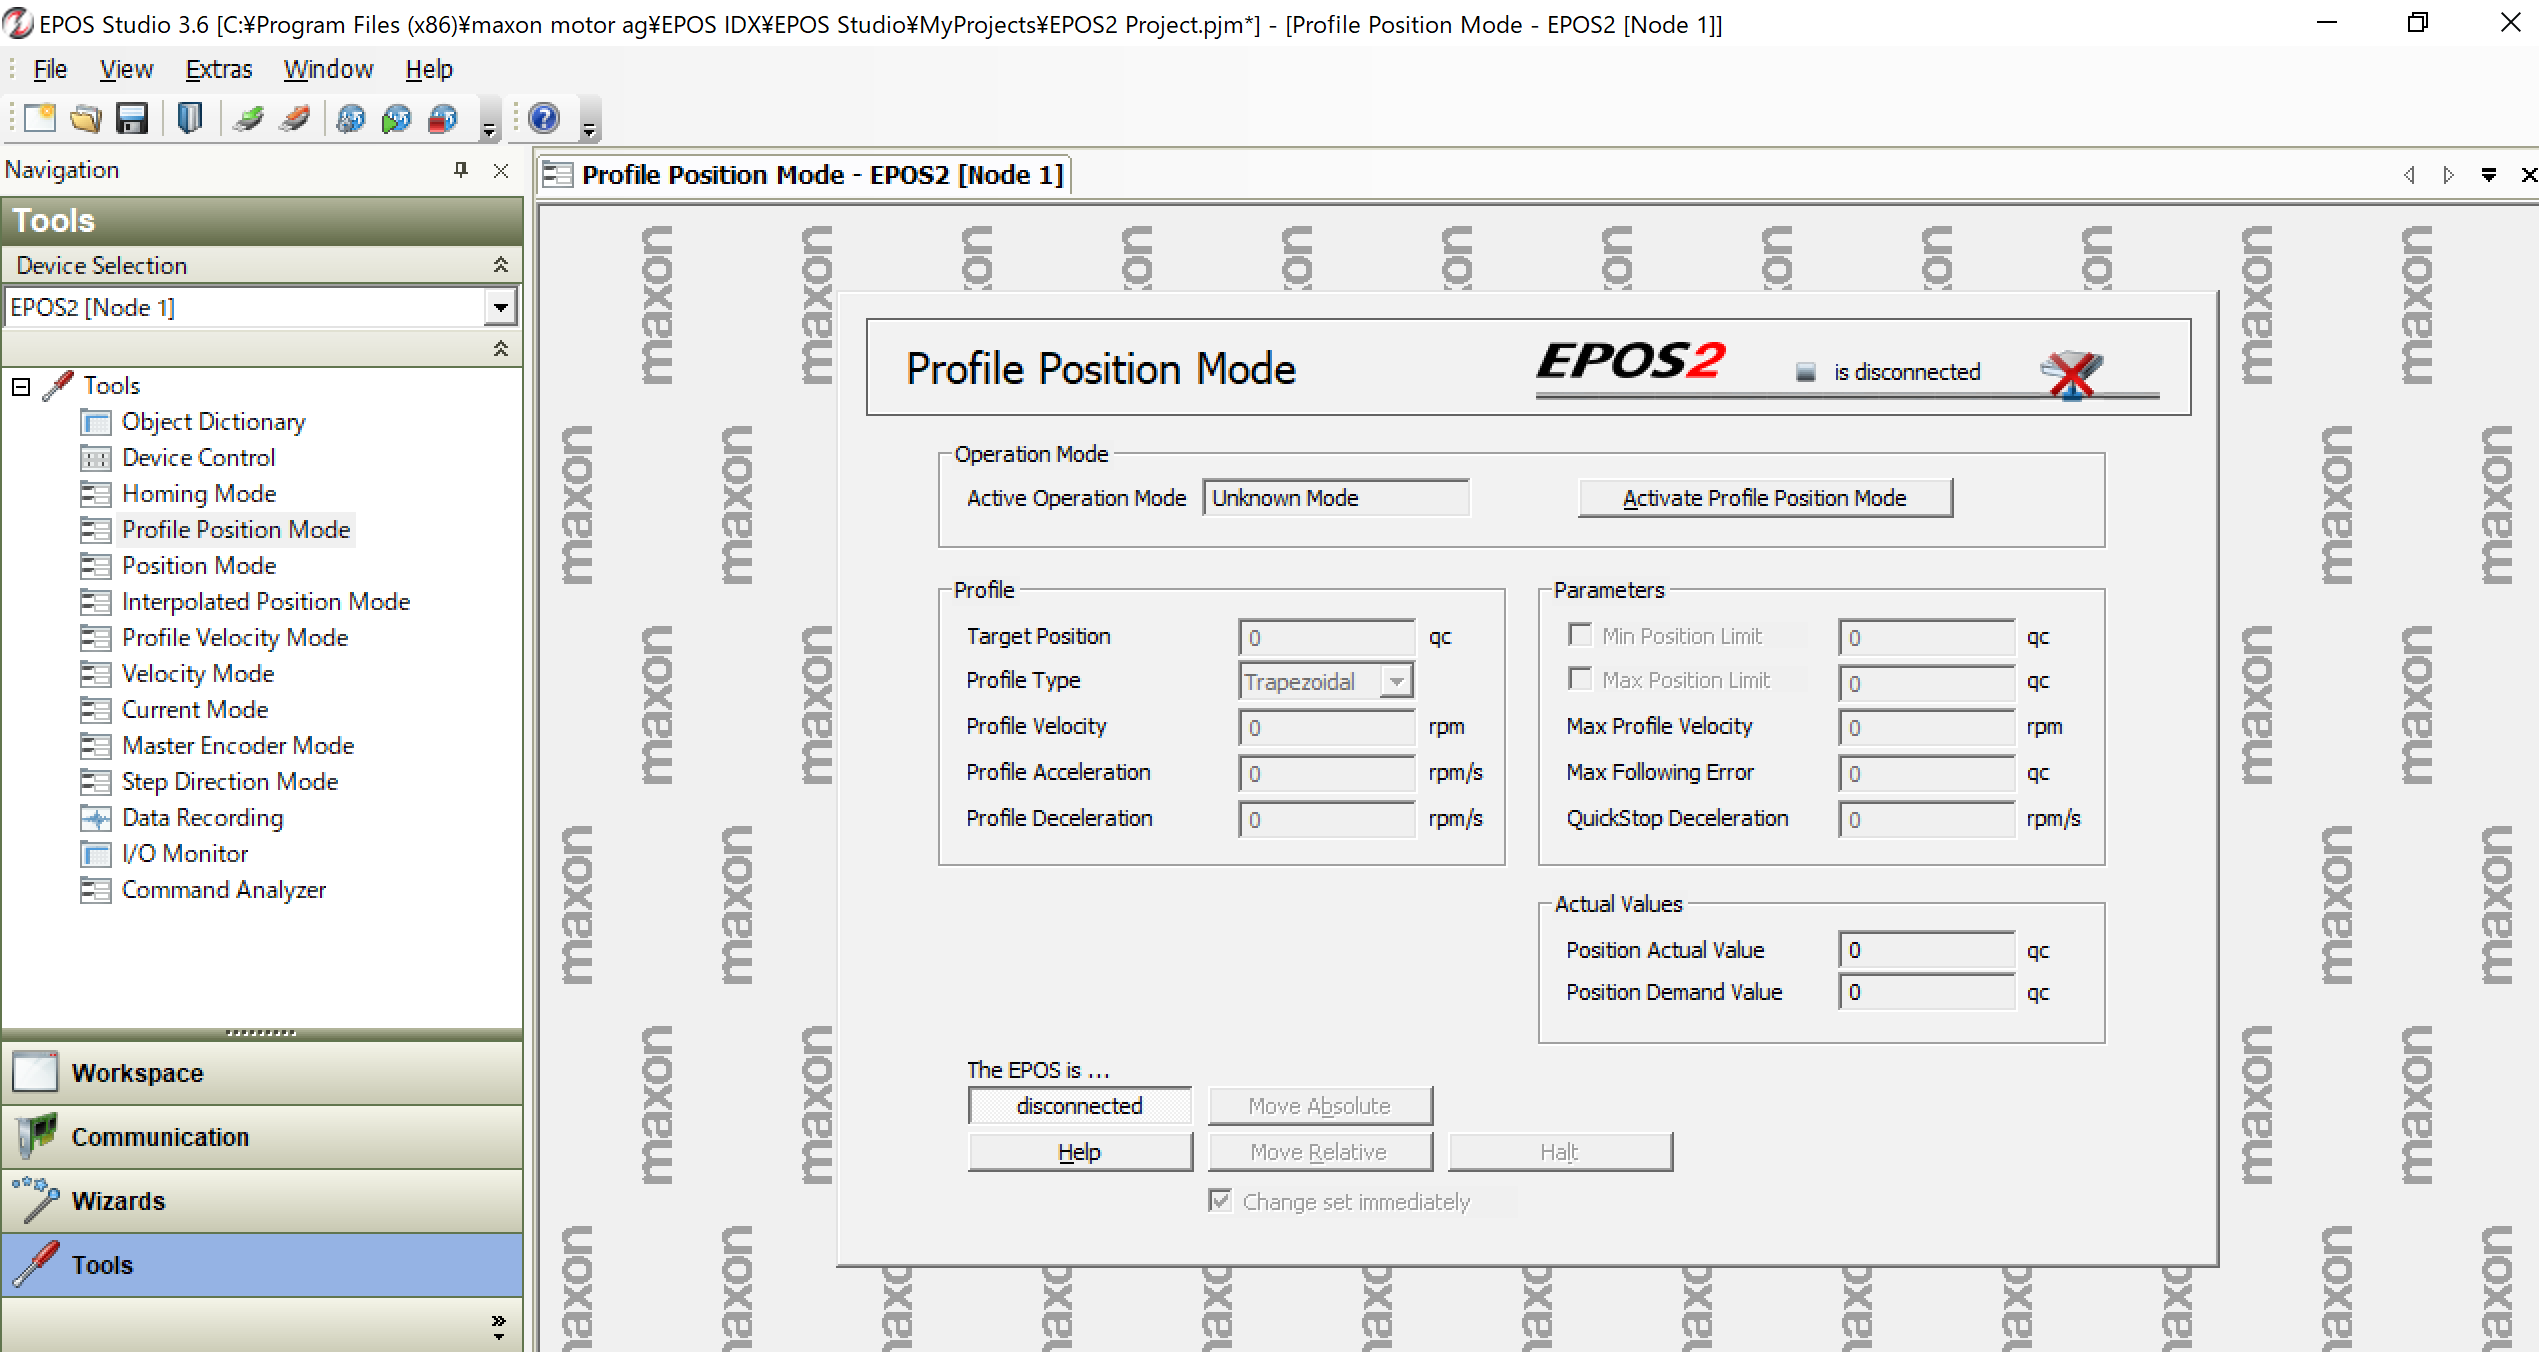
\includegraphics[height=80mm]{figure/epos_studio.eps}
    \vspace*{3mm}
    \caption{EPOS Studio}
    \label{fig:epos_studio}
  \end{center}
\end{figure}

% **************************************************
\newpage
\subsubsection{スライダクランク機構}
スライダクランク機構は回転運動を直進運動にへ変換する機構の一つである.図~\ref{fig:slider_crank}~に示すように回転するクランクとコネクティングロッドから構成される.本研究では路面の変位を±30mm確保するためにクランク長は$r=45$mm,コネクティングロッドの長さは$l=90$mmとした.クランクの回転角$\theta _{A}$とコネクティングロッド先端の変位$x_0$の関係は式(~\ref{eq:mm_to_deg}~)で表される.本研究で扱う試験では路面入力を行うために入力を変位$x_0$,出力を回転角$\theta _{A}$とする関係式が必要である.しかし式(~\ref{eq:mm_to_deg}~)では計算が複雑である.そこでLook up tableを用いた.Look up tableとはあらかじめ先に計算出来るデータを配列として入れることで配列に対応する値を参照することでデータを得る事ができ,これにより複雑な計算を効率化を可能とする.使用したsimulinkブロックを図~\ref{fig:Look}~に示す.本研究ではLook up tableの配列のデータ数は91とした.配列の要素であるクランクの回転角$\theta _{A}$の範囲は±45[°]であり,0.1[°]刻みとした.また,変位$x_0$は式(~\ref{eq:mm_to_deg}~)より計算した値となっている.
\begin{eqnarray}
 \label{eq:mm_to_deg}
x_{0} =r\times \sin \theta _{A} +\sqrt{l^{2} -r^{2}\cos^{2} \theta _{A}} -\sqrt{l^{2} -r^{2}}
 \end{eqnarray}

\vspace*{5mm}
\begin{figure}[htp]
  \begin{center}
    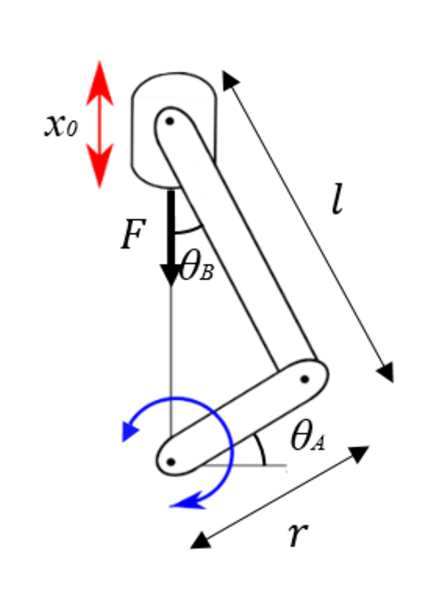
\includegraphics[height=50mm]{figure/slider_crank.eps}
    \vspace*{3mm}
    \caption{Slider Crank Mechanism}
    \label{fig:slider_crank}
  \end{center}
\end{figure}
\vspace*{5mm}
\begin{figure}[htp]
  \begin{center}
    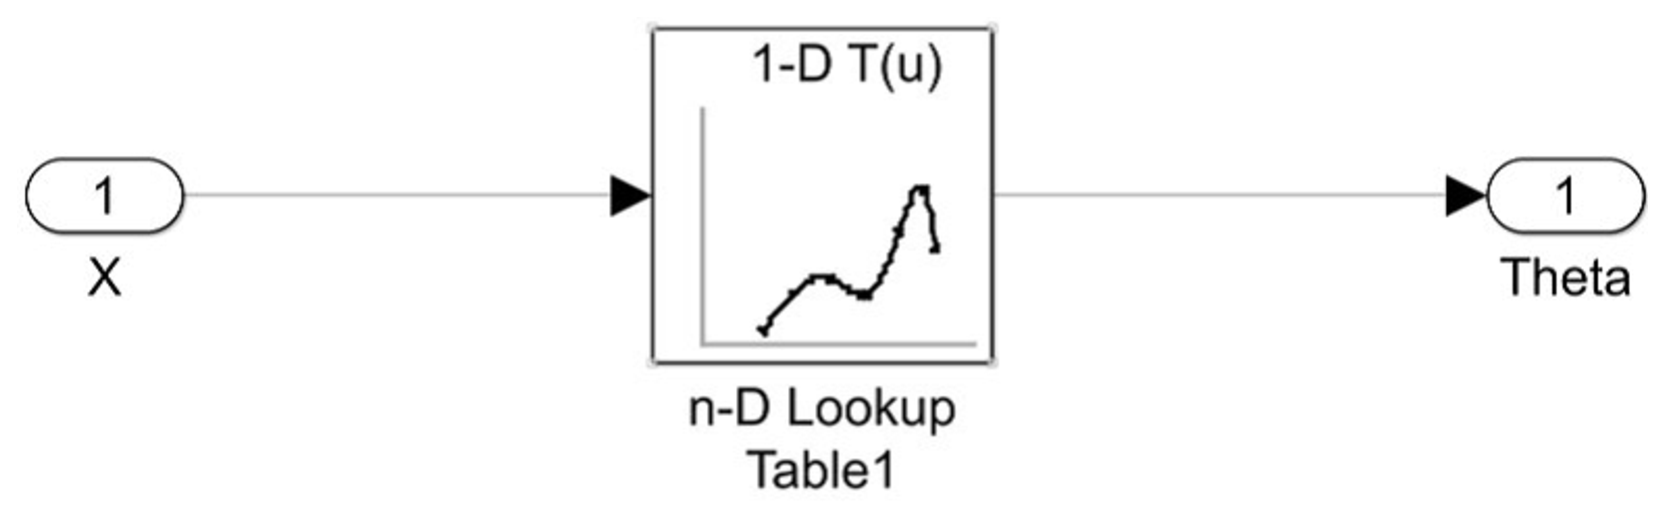
\includegraphics[height=30mm]{figure/Lookuptable.eps}
    \vspace*{3mm}
    \caption{Loou up table}
    \label{fig:Look}
  \end{center}
\end{figure}

\newpage
\subsubsection{計測機器}
本試験ではダンパが発生させる力とサスペンションストロークを計測する.
ここでは計測に用いるロードセルとレーザ変位計について説明する.
\par
まず,ロードセルについて説明する.ダンパが発生する力の計測には図~\ref{fig:tclz}~に示す東京測器研究所の引張・圧縮型高精度荷重計「TCLS-20NA」を用いた.仕様を表~\ref{tab:tclz}~に示す.このロードセルをダンパとばね上の間に取り付けることでダンパ力を計測する.ロードセルから出力された電圧値は,東京測器研究所のデジタル指示計「TD-96A」を用いて換算する.このデジタル指示計は,ひずみゲージ式変換器を用いて荷重,変位,圧力などを測定できる.外観を図~\ref{fig:td_96a}~に,仕様を表~\ref{tab:td_96a}~に示す.

\vspace*{10mm}
\begin{figure}[h!]
  \begin{tabular}{cc}
  \begin{minipage}{0.5\hsize}
  \begin{center}
    \includegraphics[height=40mm]{figure/tclz.eps}
      \vspace*{3mm}
      \caption{Loadcell(TCLZ-20NA)}
      \label{fig:tclz}
    \end{center}
  \end{minipage}
  \begin{minipage}{0.5\hsize}
     \begin{center}
      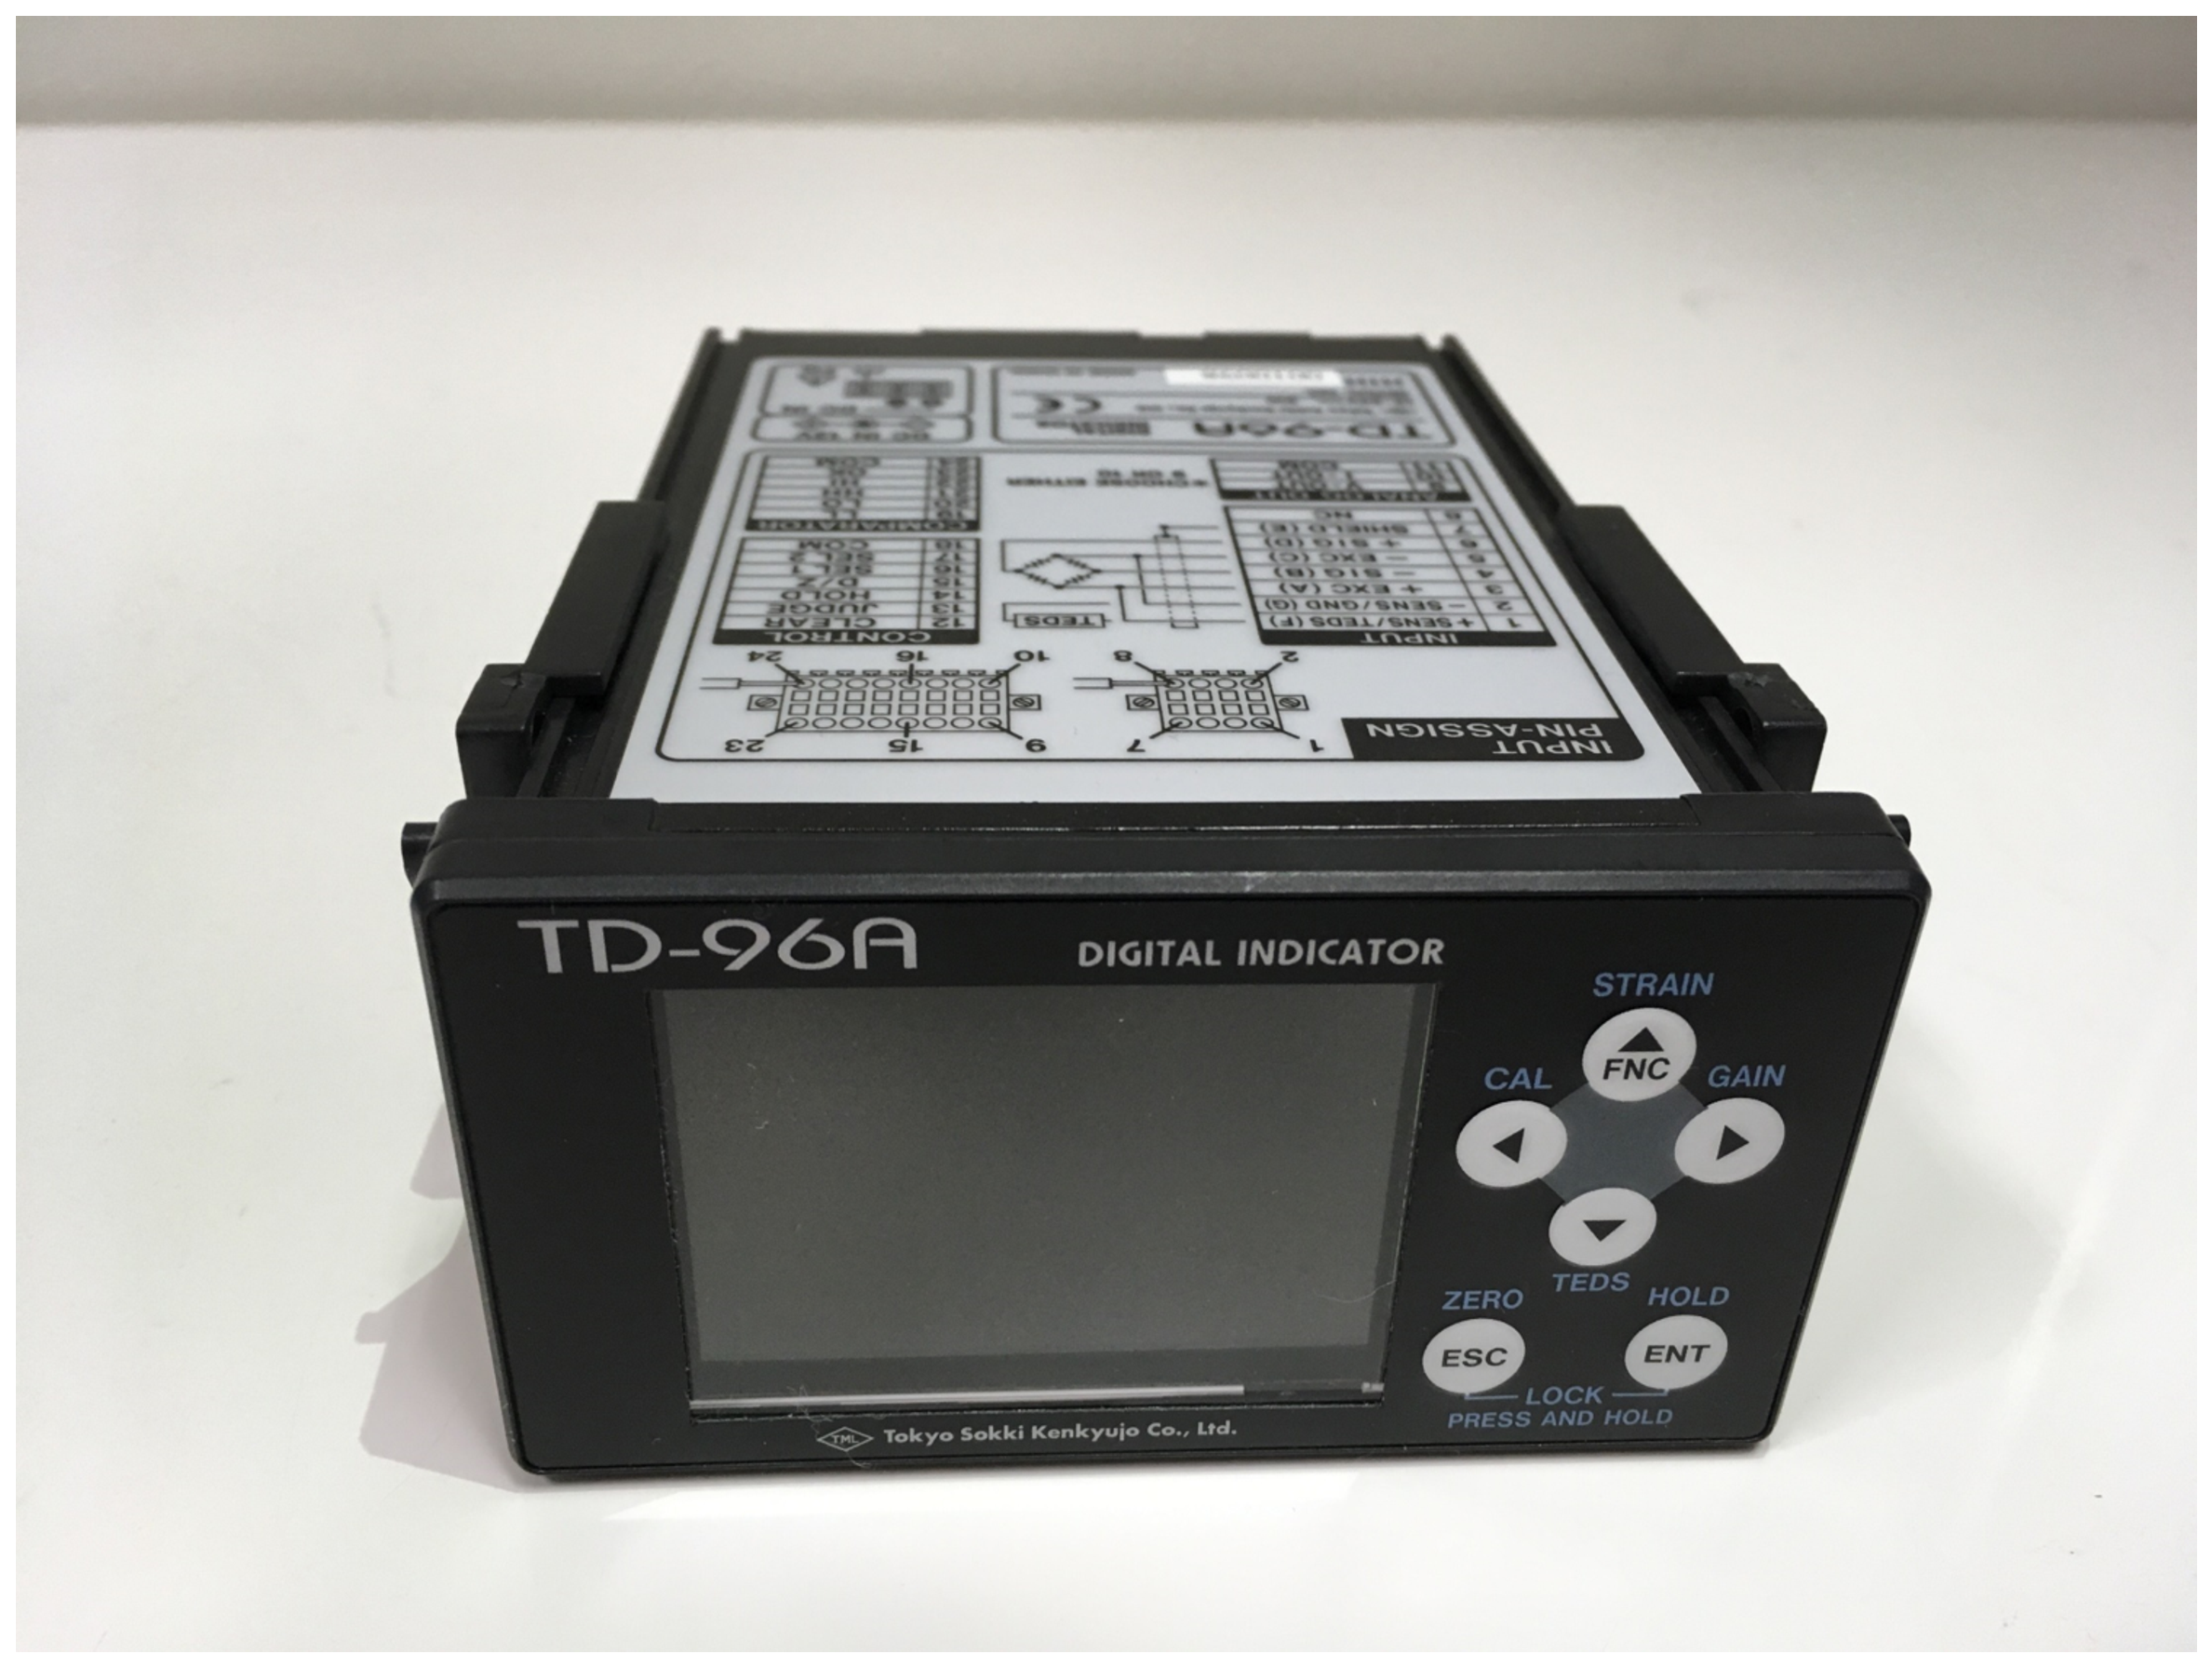
\includegraphics[height=40mm]{figure/td_96a.eps}
      \vspace*{3mm}
      \caption{Digital Indictor(TD-96A)}
      \label{fig:td_96a}
    \end{center}
  \end{minipage}
  \end{tabular}
 \end{figure}

\vspace*{10mm}
\begin{table}[h]
  \begin{center}
    \caption{Specification of Loadcell}
	\label{tab:tclz}
	\begin{tabular}{crrc}\hline
	  Parameter & \multicolumn{2}{c}{Value}&\\\hline
	  Capacity & \multicolumn{2}{c}{20 N}&\\
	  Overload Capacity & \multicolumn{2}{c}{30N}&\\
	    & Ten.&Comp.\\
	  Rated Output & +1248.7 & -1248.4 & $\mu$V/V \\
	  Strain & +2497.3 & -2496.8 & $\times$ 10$^-6$ $\epsilon$ \\
	  Calibration Coefficient & 0.008009 & 0.008010 & N/1$\times$ 10$^-6$ \\\hline
	\end{tabular}
  \end{center}
\end{table}

\vspace*{10mm}
\begin{table}[h]
  \begin{center}
    \caption{Specification of TD-96A}
    \label{tab:td_96a}
    \begin{tabular}{cc}\hline
      Measurement Point & 1 \\
      Measurement Range [mV/V]& $\pm$3\\
      A/D Conversion Speed [Hz]& 4000\\
      D/A Output [mA]& 0$\pm$1$\sim\pm$10 V, 4$\sim$20\\
      Power supply & AC100 V 12 W, DC12$\sim$24 V 9 W \\\hline
    \end{tabular}
  \end{center}
\end{table}
\newpage
  次にレーザ変位計について説明する.サスペンションストロークの計測には図~\ref{fig:il_300}~に示す株式会社KEYENCEのセンサヘッド「IL-300」を用いた.仕様を表~\ref{tab:il_300}~に示す.出力電圧は±5V,1-5V,0-5Vから選択できる.計測距離をL[mm],アナログ出力電圧をV[V]とした時,換算式はそれぞれ以下のようになる.本研究では,出力電圧±5Vの式~\ref{eq:v5}~を用いた.また,アンプとして,図~\ref{fig:il_1500}~に示す株式会社KEYENCEのアンプユニット「IL-1000」を用いた.アンプユニットには,図~\ref{fig:kz_u3}~にに示す,定電圧/定電流直流電源「LXO18-2A」を用いて12Vをアンプユニットに供給している.

\begin{eqnarray}
 \label{eq:v5} L &=& V_{\pm5V} \times 28\\
 \label{eq:v15} L &=& V_{1-5V} \times 70\\
 \label{eq:v05} L &=& V_{0-5V} \times 56
\end{eqnarray}

\vspace*{10mm}
\begin{figure}[htp]
  \begin{minipage}{0.3\textwidth}
    \begin{center}
      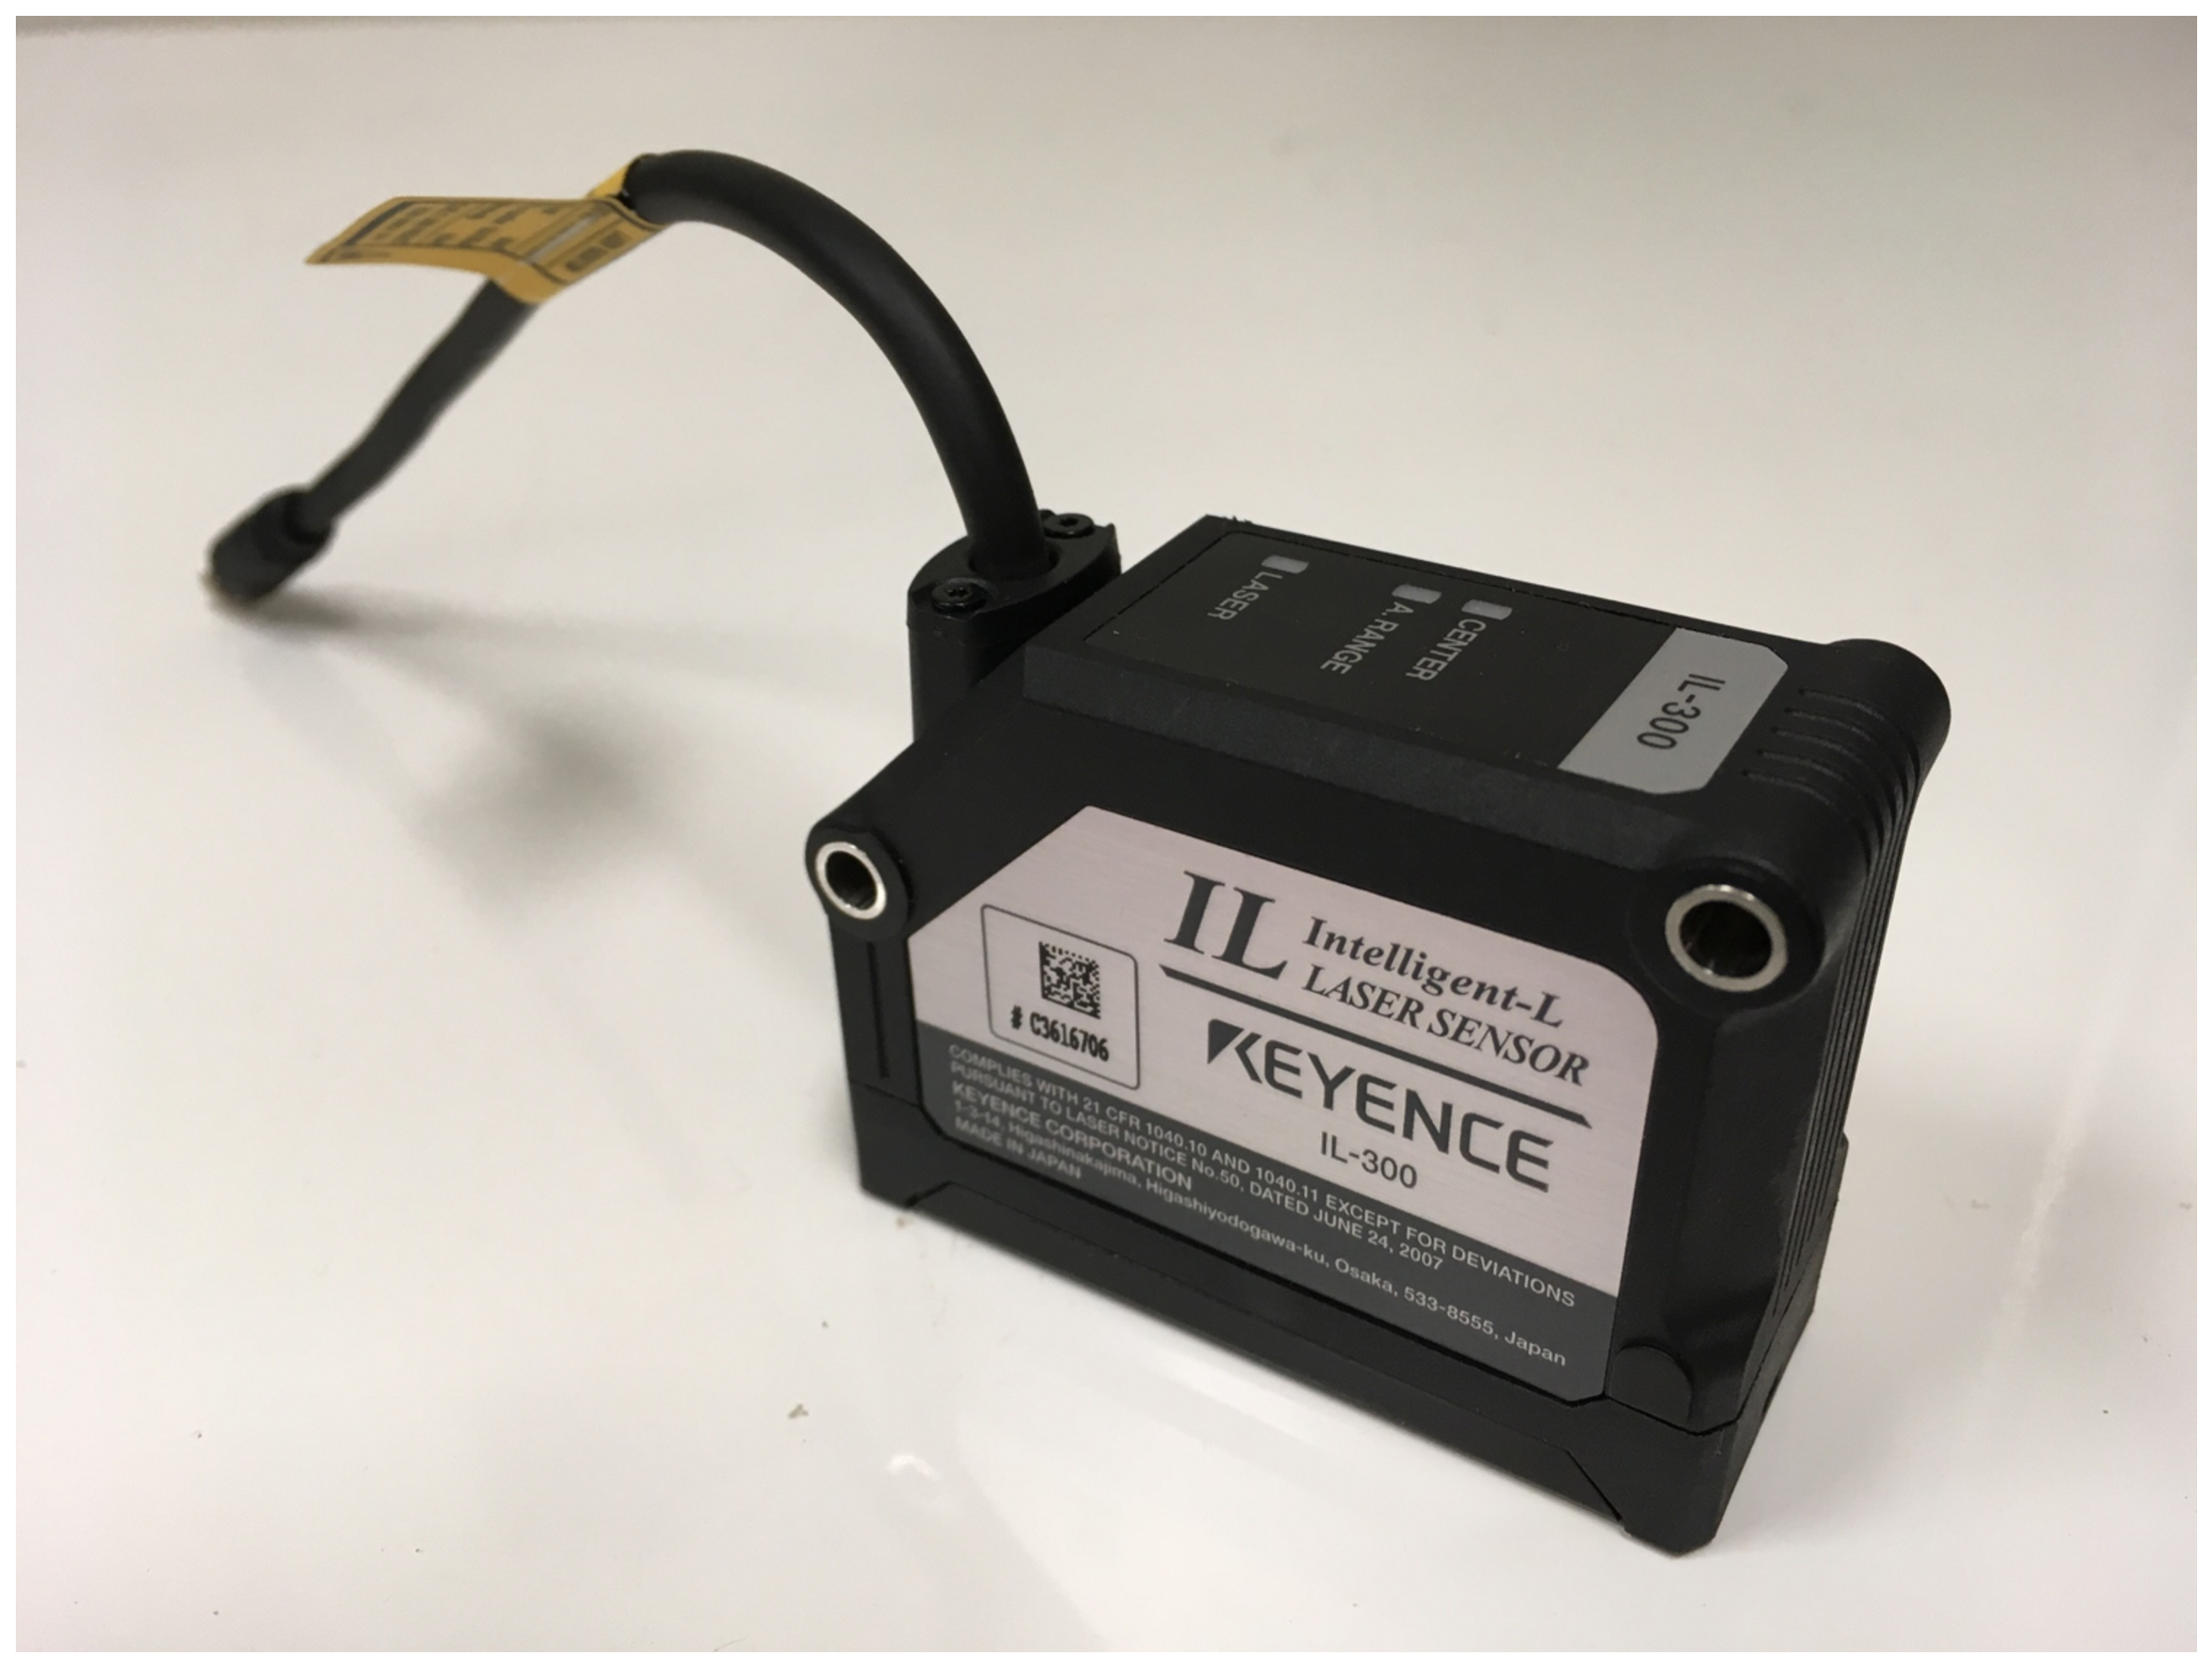
\includegraphics[height=40mm]{figure/il_300.eps}
      \vspace*{3mm}
      \caption{Laser Displacement Sensor(IL-300)}
      \label{fig:il_300}
    \end{center}
  \end{minipage}
  \begin{minipage}{0.7\textwidth}
      \begin{center}
	\makeatletter
	\def\@captype{table}
	\makeatother
	\caption{Specification of Laser Displacement Sensor}
	\label{tab:il_300}
	\begin{tabular}{ccc}\hline
	  Measurement Center Distance [mm] & 300\\
	  Measuring Range & 160-450 mm\\
	  Sampling Period [$\mu$s]& 0.33 / 1 / 2 / 5\\
	  Resolition [$\mu$m] & 10\\
	  Linearity [\%F.S.] & $\pm$0.25\\
	  Receiving Element & Liner Image Sensor\\
	  Resistance to Vibration [Hz] & 10-55\\
	  Laser Class & 2\\
	  Power Supply & DC10-30 V\\\hline
	  \end{tabular}
	\end{center}
  \end{minipage}
\end{figure}

\vspace*{10mm}
\begin{figure}[htp]
  \begin{minipage}{0.5\textwidth}
    \begin{center}
      \includegraphics[height=40mm]{figure/IL_1000.eps}
      \vspace*{3mm}
      \caption{Amplifier Unit(IL-1000)}
      \label{fig:il_1500}
    \end{center}
  \end{minipage}
  \begin{minipage}{0.5\textwidth}
    \begin{center}
      \includegraphics[height=40mm]{figure/LXO18-2A.eps}
      \vspace*{3mm}
      \caption{Power Supply Unit(LXO18-2A)}
      \label{fig:kz_u3}
    \end{center}
  \end{minipage}
\end{figure}


\newpage
\subsection{ソフトウェア}
\subsubsection{dSPACEシステム}
本システムでは,dSPACE社製の開発環境であるdSPACEシステムを利用している.上下変位計算とハードウェア制御にはdSPACE社製のController Board「DS1104 Controller Board」を使用している.Controller Boardを図~\ref{fig:ds1104}~に,Connector Panelを図~\ref{fig:conpane}~に示す.Controller Boardは,デジタル入出力用チャンネル,A/Dコンバータ用チャンネル,D/Aコンバータ用チャンネルを備えており,多くの用途に対応できる.また,Digital Incremental Encorder Interface用チャンネルによるエンコーダの計測や,Serial Interfaceに対応しておりボーレート最大115200bpsのRS232通信が可能である.

\vspace{10mm}
\begin{figure}[h]
    \begin{tabular}{c}
      \begin{minipage}{0.5\hsize}
	\begin{center}
	  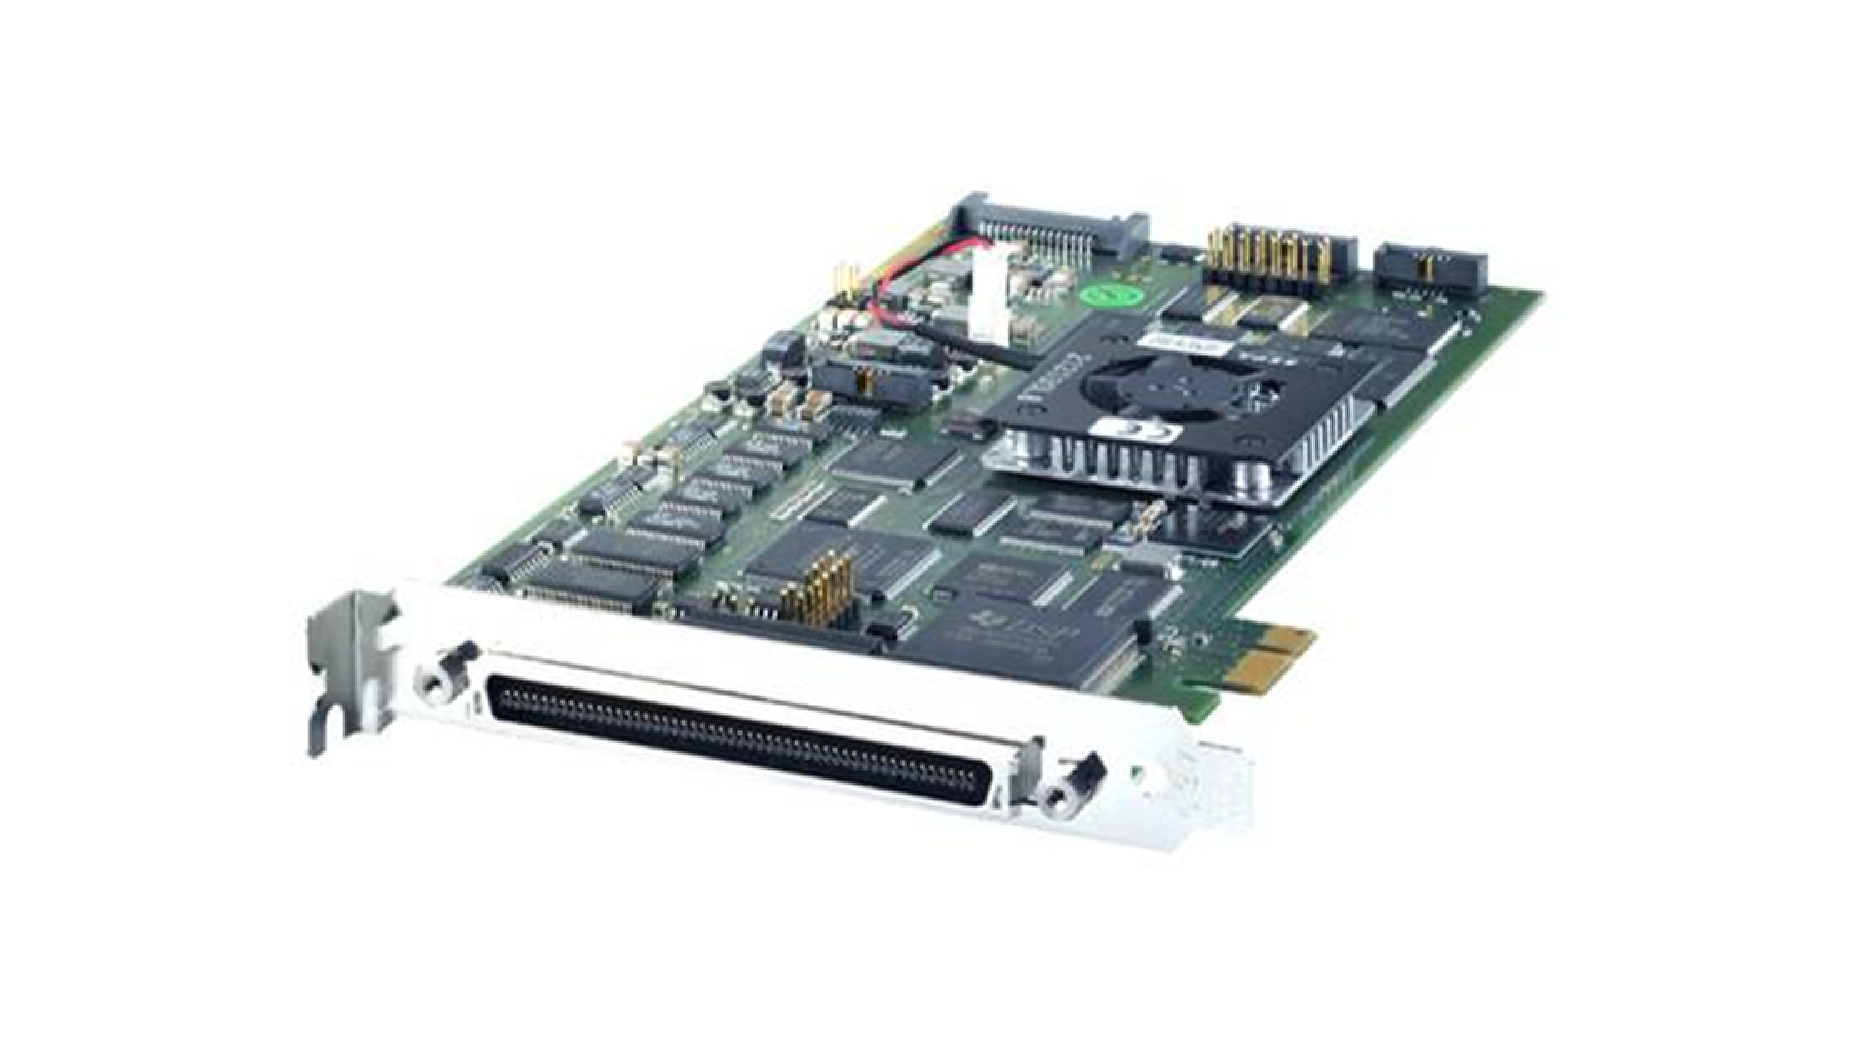
\includegraphics[height=25mm]{figure/ds1104.eps}
	  \caption{Controller Borad\cite{66}}
	  \label{fig:ds1104}
	\end{center}
      \end{minipage}
      \begin{minipage}{0.5\hsize}
	\begin{center}
	  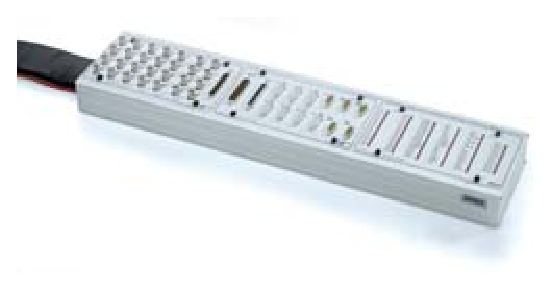
\includegraphics[height=25mm]{figure/conpane.eps}
	  \caption{Connector Panel\cite{66}}
	  \label{fig:conpane}
	\end{center}
      \end{minipage}
    \end{tabular}
\end{figure}

\vspace{10mm}
Real-Time Interfaceは,dSPACE社製のハードウェアとMathWorks社製のソフトウェア「MATLAB /Simulink」の間のリンクとなるものである.これにより,Simulinkモデルを用いてdSPACEシステムの入出力機器と信号処理を行うことができる.また,MATLAB/Simulinkで作成されたモデルは,Simulink Corderにより,実時間で実行可能なCコードに変換され,Controller Board上で実行される.このような開発環境を構築することで,実時間シミュレーションを行うHILSシステムを実現している.制御インターフェースとしては,dSPACE社製のControl Deskを用いている.「MATLAB/Simulink」と関連付けることで,試験条件の設定やハードウェアへの指令値,計測値,車両運動解析の結果をモニタリングできる.また,リアルタイムで計測値や解析結果をグラフとして描画できる.図~\ref{fig:control_desk}~では指令値や計測値,上下変位計算の結果を表示したControl Deskの画面である.

 \vspace{10mm}
\begin{figure}[h]
  \centering
  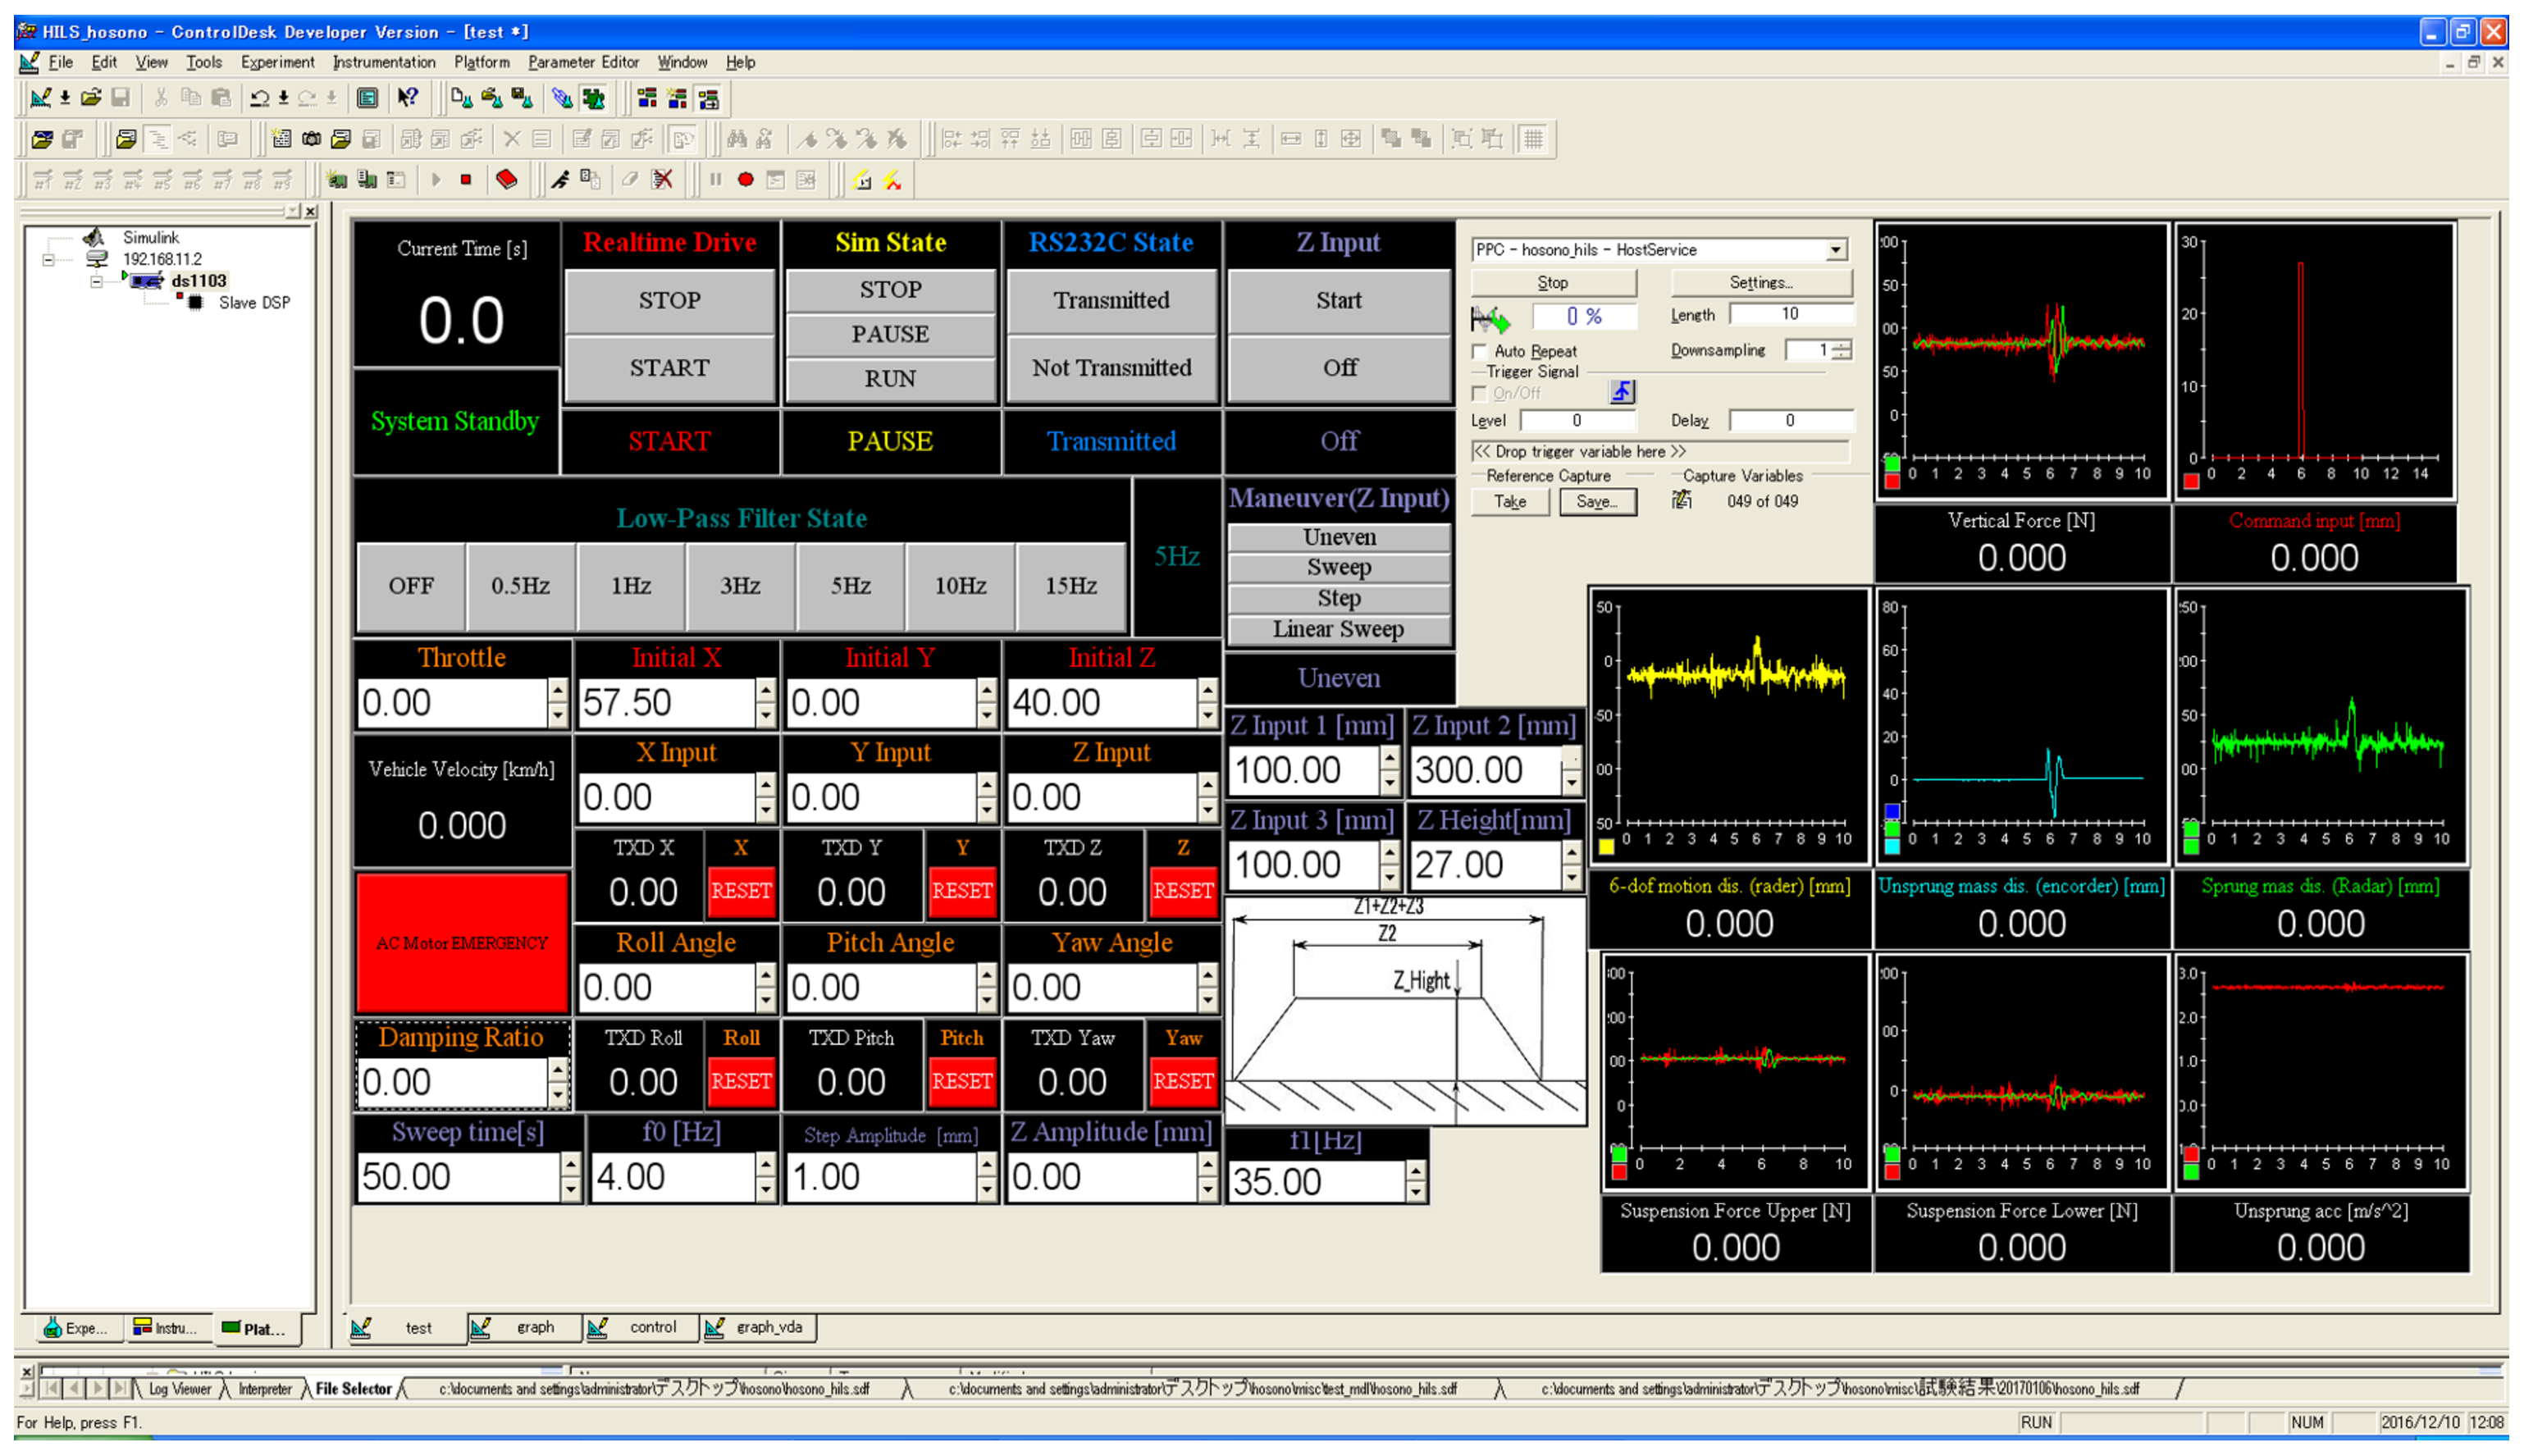
\includegraphics[height=30mm]{figure/control_desk.eps}
  \vspace{2mm}
   \caption{Control Desk}
  \label{fig:control_desk}
\end{figure}


\subsubsection{解析モデル}
本システムにおいて解析モデルは上下2自由度モデルを用いた.上下2自由度モデルは車両の上下動を表すことのできるモデルのひとつである\cite{7}.モデル図を図~\ref{fig:analysis_model}~に,諸元を表~\ref{tab:parameter}~に示す.また,このモデルの運動方程式は以下である.

\begin{eqnarray}
 \label{eq:2dof_m1} &&m_1\ddot x_1 + k_1(x_1-x_0) + k_2(x_1-x_2) - f_c = 0\\
 \label{eq:2dof_m2} &&m_2\ddot x_2 + k_2(x_2-x_1) + f_c = 0
\end{eqnarray}

\vspace{10mm}
ここで,$m_1$はばね下質量 ,$m_2$はばね上質量,$k_1$,$k_2$はばね定数,$c_2$は減衰係数,$x_0$は路面変位,$x_1$はばね下変位,$x_2$はばね上変位である.そして,$f_c$はHILS試験機で計測されたダンパ力を用いる.

\vspace*{10mm}
\begin{figure}[htp]
  \begin{minipage}{0.5\textwidth}
    \begin{center}
      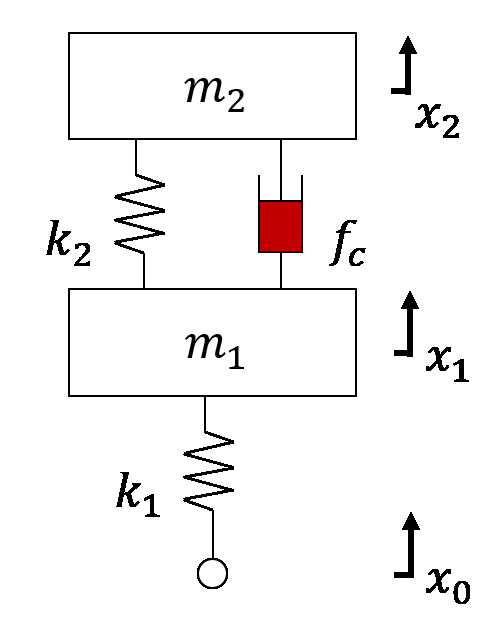
\includegraphics[height=40mm]{figure/analysis_model.eps}
      \vspace*{3mm}
      \caption{Analysis Model}
      \label{fig:analysis_model}
    \end{center}
  \end{minipage}
  \begin{minipage}{0.5\textwidth}
      \begin{center}
	\makeatletter
	\def\@captype{table}
	\makeatother
	\caption{Parameter of Analysis Model}
	\label{tab:parameter}
	  \begin{tabular}{cc}\hline
	    Unsprung Mass $m_1$ [kg] & 1.5\\
	    Sprung Mass $m_2$ [kg] & 6.9\\
	    Spring constant $k_1$ [N/m] & 2200\\
	    Spring constant $k_2$ [N/m] & 439\\\hline
	  \end{tabular}
	\end{center}
  \end{minipage}
\end{figure}

\newpage
\subsection{HILSシステムの概要}
本研究室で開発されたHILSシステムの概要を図~\ref{fig:HILS}~に示す.HILSシステムは,ハードウェアある試験装置と,ソフトウェアである車両運動解析やシステム制御を行うPCから構成される.本システムでは試験装置から計測されたダンパ力を用いてリアルタイム車両運動解析を実行し,サスペンションストロークを算出する.この解析結果の基づきアクチュエータを制御することでリアルタイムに車両の上下動を再現している.
\vspace*{10mm}
\begin{figure}[htp]
  \begin{center}
    \includegraphics[height=80mm]{figure/HILS1.eps}
    \vspace*{3mm}
    \caption{Tire-Suspension HILS System}
    \label{fig:HILS}
  \end{center}
\end{figure}
\vspace*{10mm}
\newpage
\section{アクチュエータの制御手法}
ここではアクチュエータへの制御手法について説明する.アクチュエータへの入力$\bar{x}_0$は解析モデルの計算結果に基づき決定する.解析モデルは上下2自由度振動系であるのに対し、本研究室で扱うHILS試験機はばね上が固定された1自由度振動系である.2自由度振動系の上下変位$x_2-x_1$は,1自由度振動系の$-\bar{x}_1$に相当する.自由度が異なるため、解析モデルの入力である路面変位$x_0$をHILS試験機のアクチュエータの入力$\bar{x}_0$とすることはできない.そのため,路面変位を解析モデルへ入力し,計算された上下変位$x_2-x_1$と試験機の$-\bar{x}_1$が一致するようにアクチュエータを制御する.HILSシステムのブロック線図を図~\ref{fig:1dof_block}~に示す.

\begin{figure}[htp]
  \begin{center}
    \includegraphics[height=45mm]{figure/Block_Diagram_A.eps}
    \vspace*{3mm}
    \caption{Block Diagram}
    \label{fig:1dof_block}
  \end{center}
\end{figure}
\subsection{相対変位による制御手法}
ここではアクチュエータへの制御手法として相対変位を用いた手法について説明する.ブロック線図を図~\ref{fig:1dof_Relative_moedel_block}~に示す.アクチュエータへの入力$\bar x_0$は解析モデルを用いて計算した車体-路面間相対変位$x_2-x_0$に基づき決定する.

\vspace*{10mm}
\begin{figure}[htp]
  \begin{center}
    \includegraphics[height=45mm]{figure/Block_Diagram_t_r.eps}
    \vspace*{3mm}
    \caption{Block Diagram(Relative)}
    \label{fig:1dof_Relative_moedel_block}
  \end{center}
\end{figure}
\newpage
\subsection{逆伝達関数による制御手法}
ここではアクチュエータへの制御手法として逆伝達関数を用いた手法について説明する.解析モデルの上下変位$x_2-x_1$は,試験機の$-\bar{x}_1$に相当する.そこで試験機を図~\ref{fig:1DOF}~のような1自由度振動系としてモデル化し,入力$\bar{x}_0$に対する出力$-\bar{x}_1$の逆伝達関数を考慮してアクチュエータへの入力を決定する.このとき,逆モデルの計算を行うためダンパは線形とし,装置の周波数応答から$c_2$をパラメータ同定した.ハードウェアの諸元を表~\ref{tab:1DOF}~に示す.運動方程式は式~(\ref{eq:1DOF})~ に示す.逆伝達関数を用いた制御手法のブロック線図を図~\ref{fig:1dof_Invere_model_block}~に示す.

\vspace*{-10mm}
\begin{flalign}
\label{eq:1DOF}
\ & m_1\ddot{\bar{x}}_1+c_2\dot{\bar{x}}_1+k_1(\bar{x}_1-\bar{x}_0)+k_2\bar{x}_1=0
\end{flalign}

\vspace{-2mm}
ここで,$m_1$はばね下質量 ,$m_2$はばね上質量,$k_1$はタイヤの縦ばね剛性,$k_2$はばね定数,$c_2$は減衰係数,$\bar{x}_0$はHILS試験機の路面部変位,$\bar{x}_1$はばね下部変位である.

\vspace{10mm}
\begin{figure}[h]
  \begin{minipage}{0.3\hsize}
     \begin{center}
      \includegraphics[height=35mm]{figure/inverse_model.eps}
	\vspace{2mm}
      \caption{Hardware Model}
      \label{fig:1DOF}
    \end{center}
  \end{minipage}
\begin{minipage}{0.65\hsize}
\makeatletter
\def\@captype{table}
\makeatother
  \begin{center}
   \caption{Parameter of 1DOF Model}
   \label{tab:1DOF}
   \begin{tabular}{cc}\hline
      Unsprung Mass $m_1$ [kg] & 1.5  \\
      Vertical spring stiffness $k_1$ [N/m] & 2200  \\
      Spring constant $k_2$ [N/m] & 439   \\
      Damping coefficient $c_2$ [N/m] & 15   \\ \hline
    \end{tabular}
   \end{center}
 \end{minipage}
\end{figure}
\vspace*{10mm}
\begin{figure}[htp]
  \begin{center}
    \includegraphics[height=45mm]{figure/Block_Diagram_t_i.eps}
    \vspace*{3mm}
    \caption{Block Diagram(Inverse Transfanc)}
    \label{fig:1dof_Invere_model_block}
  \end{center}
\end{figure}
% \subsubsection{フィルタの検討}

\newpage
\subsection{摩擦の影響を考慮した制御手法}
\subsubsection{等価粘性減衰係数を用いた摩擦力の影響}
一般に機械摩擦は,図~\ref{fig:Fric}~のような運動方向の変化に応じて,急激に変化する非線形な特性を有する.
特に,速度反転時や低速度領域の,非線形な摩擦挙動は,機械システムの運動特性に大きな影響を与える.
微小な運動領域では,摩擦力は,ばねのような特性を示し,変位と摩擦力の関係がヒステリシスループを描くことが知られている\cite{hys1}.
このような摩擦力は,タイヤ-サスペンション試験機のサスペンション部にも存在しており,HILSシステムの再現性に影響を与えることが考えられる.
\par
摩擦を解析で考慮する場合,摩擦力によるエネルギ損失を等価な粘性減衰に置き換える手法がある.この時,設定される減衰係数を等価減衰係数もしくは等価粘性減衰定数と呼ぶ.
粘性減衰は振動解析上,最も基本的な減衰であり,減衰系で発生する減衰力は相対速度に比例する.すなわち減衰力を$F$,相対速度を$v$とすると,$F=cv$と表せる.
等価減衰係数は,同一の振動系においても振幅や周波数などの振動の条件によって適値が変化してしまうが,適切に設定することで減衰要素の解析を容易に行うことができる.

本研究においては,解析モデルで計算されたストローク速度と,等価減衰係数をかけることでサスペンション部の摩擦力の影響を解析モデル内に考慮した.解析モデルを図~\ref{fig:model_GD}~に示す.

\vspace*{5mm}
\begin{figure}[h]
  \begin{center}
    \includegraphics[scale = 0.3]{figure/friction_image.eps}
    \vspace*{3mm}
    \caption{Friction Force Based on Velocity}
    \label{fig:Fric}
  \end{center}
\end{figure}
\begin{figure}[h]
  \begin{center}
    \includegraphics[height=40mm]{figure/model_GD.eps}
    \vspace*{3mm}
    \caption{Analysis Model Include Friction Effect}
    \label{fig:model_GD}
  \end{center}
\end{figure}
\newpage
\subsubsection{等価粘性減衰係数の適応同定}
先述したように,摩擦力に対応する等価減衰係数は試験機の挙動に応じて変化する.
そこで本研究では,等価粘性減衰係数の適応同定を行うことで,解析モデルの精度向上および~HILS~システムの再現性向上を図った.

適応同定および適応制御とは,環境状況や動作条件の変動により制御対象の特性が大きく変化する場合において,制御対象のモデル内に存在する変動パラメータに応じて制御器の特性を自動調整する手法である\cite{tt}.
本研究では解析モデルと試験機の計測結果を含む評価関数を設計した.この評価関数は解析モデルと試験機の計測結果の差を表している.評価関数が小さくなるような等価粘性減衰係数を算出するという方式をとった.
使用した評価関数を以下に示す.

\vspace{-2mm}
\begin{equation}
J=\frac{1}{2}\ \{w_v(\dot{x}_H-\dot{x}_M)^2 + w_p(x_H - x_M)^2 + w_c(c^{(k)}_f - c^{(k-1)}_f)^2\}
\end{equation}
ここで
$x_H$,$x_M$~は試験機および解析モデルのサスペンションストローク,
$c_f$~は等価減衰係数,
$c_0$~は等価減衰係数の初期値である.
また,
$w_v$は試験機と解析モデルのサスペンションストローク速度の差に対する重みづけ係数,
$w_p$は試験機と解析モデルのサスペンションストロークの差に対する重みづけ係数,
$w_c$は等価粘性減衰係数の変化量に対する重みづけ係数である.

\subsubsection{評価関数の最小化}
本研究において評価関数の最小化には勾配法の一種である最急降下法を使用した.
最急降下法とは関数の最小値を探索するアルゴリズムの一つであり,ドライビングシミュレータにおけるモーションキューイングなど,リアルタイム性を重視するハードウェアの制御に用いられている\cite{MC}.

P の関数 J においては初期値を基に式 \ref{steep} を反復することで P の値を更新していく.

\vspace{-2mm}
\begin{eqnarray}
 c^{(k+1)}_{f} = c^{(k)}_{f} - \gamma \cdotp \frac{\partial J}{\partial c_{f}}
 \label{steep}
\end{eqnarray}
$\frac{\partial J}{\partial c_{f}}$ が十分小さな値となったときの J が極小値である.
$\gamma$ は収束速度に関わるパラメータである.
$\gamma$ は大きすぎると発散する可能性があり,小さいと収束が遅くなる.
関数の傾きから計算するため計算速度は早いが,局所的な最小値に陥りやすいという特徴がある.
\newpage
\subsubsection{評価関数の偏微分}
本研究で扱った式 (\ref{steep1})について説明する.
まずはじめに$\frac{\partial J}{\partial c_{f}}$ について解説する.$\frac{\partial J}{\partial c_{f}}$ は式 (\ref{steep_1})のように展開できる.

\begin{eqnarray}
 c^{(k+1)}_{f} = c^{(k)}_{f} - \gamma \cdotp \frac{\partial J}{\partial c_{f}}
 \label{steep1}
\end{eqnarray}
%
\begin{eqnarray}
  \frac{\partial J}{\partial c_{f}} \ =\ w_{p}( x_{h} -x_{s})\frac{\partial x}{\partial c_{f}} +w_{v}(\dot{x}_{h} -\dot{x}_{s})\frac{\partial \dot{x}}{\partial c_{f}} +w_{c}( c^{(k)}_{f} -c^{(k-1)}_{f})
 \label{steep_1}
\end{eqnarray}

ここで式 \ref{steep_1}の$\frac{\partial x}{\partial c_{f}}$と$\frac{\partial \dot{x}}{\partial c_{f}}$
は一自由度振動計の運動方程式\ref{steep_2}を変換することで算出することができる.モデル図を図\ref{fig:model_GD}に示す.$\frac{\partial x}{\partial c_{f}}$を式\ref{steep_3},$\frac{\partial \dot{x}}{\partial c_{f}}$を式\ref{steep_4}に示す.

\begin{eqnarray}
 m_{1}\ddot{x}_{1} +( k_{1} +k_{2}) x_{1} +c_{2}\dot{x}_{1} +f_{c} -k_{1} x_{0} \ =\ 0
 \label{steep_2}
\end{eqnarray}


\begin{eqnarray}
\frac{\partial x}{\partial c_{f}} \ =\ -\frac{1}{k_{1} +k_{2}}\dot{x}_{1}
\label{steep_3}
\end{eqnarray}

\begin{eqnarray}
\frac{\partial \dot{x}}{\partial c_{f}} \ =\ -\frac{1}{c^{2}_{f}}\{m_{1}\ddot{x}_{1} +( k_{1} +k_{2}) x_{1} -f_{c} -k_{1} x_{0}\}
\label{steep_4}
\end{eqnarray}

\begin{figure}[h]
  \begin{center}
    \includegraphics[height=40mm]{figure/model_1.eps}
    \vspace*{3mm}
    \caption{1DOF}
    \label{fig:model_1dof_GD}
  \end{center}
\end{figure}
しかし本研究では,試験機の変位はレーザ変位計,ダンパ力はロードセルにより計測するため計測結果にノイズがのってしまい値にバラツキが出てしまう.そこで本研究のHILS試験では式\ref{steep_3},\ref{steep_4}は簡易化し,定数として扱う.シミュレーション結果にて式\ref{steep_3},\ref{steep_4}を用いて計算を行い,検証を行う.

\newpage
\section{制御手法によるHILSシステムの影響}
\subsection{シミュレーション}
HILSシステムにで試験する前にハードウェアを1自由度モデルに置き換えたシミュレーションを行った.この時の相対変位による制御手法のブロック線図を図~\ref{fig:sim_rel}~,逆伝達関数によるアクチュエータの制御のブロック線図を図~\ref{fig:sim_inv}~に示す.解析モデルで計算したサスペンションストロークとハードウェアのモデルで計算したサスペンションストロークの結果を比較する.今回はHILS試験機サスペンションストローク範囲が25mmであるためその範囲を超えない上でシミュレーションを行う.ハードウェアのモデルは3.2節で述べたモデルを使用する.

\vspace*{10mm}
\begin{figure}[htp]
  \begin{center}
    \includegraphics[height=50mm]{figure/Block_Diagram_t_r_sim.eps}
    \vspace*{3mm}
    \caption{Block Diagram(Relative)}
    \label{fig:sim_rel}
  \end{center}
\end{figure}
\vspace*{10mm}
\begin{figure}[htp]
  \begin{center}
    \includegraphics[height=50mm]{figure/Block_Diagram_t_i_sim.eps}
    \vspace*{3mm}
    \caption{Block Diagram(Inverse Transfanc)}
    \label{fig:sim_inv}
  \end{center}
\end{figure}

\newpage
図~\ref{fig:sim_5_3}に周波数3.0Hz,振幅5mmの正弦波を路面入力,図~\ref{fig:sim_3_5}~に周波数5.0Hz,振幅3mmの正弦波入力,図~\ref{fig:sim_2_7}~に周波数7.0Hz,振幅2mmの正弦波入力した際の,サスペンションストロークを比較したグラフを示す.路面入力に対する二つの制御手法でのサスペンションストロークを示す.解析モデルで計算したサスペンションストロークとハードウェアのモデルで計算した結果を示す.
シミュレーション結果より,逆伝達関数による制御手法においてはフィルタのよる遅れが確認できた.

\vspace*{10mm}
\begin{figure}[h]
  \begin{tabular}{cc}
  \begin{minipage}{0.5\hsize}
  \begin{center}
    \includegraphics[height=35mm]{figure/5_3_rel.eps}
    \end{center}
    \begin{center}
    \ (a)Relative\
    \end{center}
  \end{minipage}
  \begin{minipage}{0.5\hsize}
     \begin{center}
      \includegraphics[height=35mm]{figure/5_3_inv.eps}
      \end{center}
      \begin{center}
      \ (b)Inverse Transfanc\
    \end{center}
  \end{minipage}
  \end{tabular}
  \vspace*{3mm}
  \caption{Comparison of Suspension Stroke(Input:3Hz 5mm)}
    \label{fig:sim_5_3}
\end{figure}
\begin{figure}[h]
  \begin{tabular}{cc}
  \begin{minipage}{0.5\hsize}
  \begin{center}
    \includegraphics[height=35mm]{figure/3_5_rel.eps}
    \end{center}
    \begin{center}
    \ (a)Relative\
    \end{center}
  \end{minipage}
  \begin{minipage}{0.5\hsize}
     \begin{center}
      \includegraphics[height=35mm]{figure/3_5_inv.eps}
      \end{center}
      \begin{center}
      \ (b)Inverse Transfanc\
    \end{center}
  \end{minipage}
  \end{tabular}
  \vspace*{3mm}
  \caption{Comparison of Suspension Stroke(Input:5Hz 3mm)}
    \label{fig:sim_3_5}
\end{figure}
\begin{figure}[h]
  \begin{tabular}{cc}
  \begin{minipage}{0.5\hsize}
  \begin{center}
    \includegraphics[height=35mm]{figure/2_7_rel.eps}
    \end{center}
    \begin{center}
    \ (a)Relative\
    \end{center}
  \end{minipage}
  \begin{minipage}{0.5\hsize}
     \begin{center}
      \includegraphics[height=35mm]{figure/2_7_inv.eps}
      \end{center}
      \begin{center}
      \ (b)Inverse Transfanc\
    \end{center}
  \end{minipage}
  \end{tabular}
  \vspace*{3mm}
  \caption{Comparison of Suspension Stroke(Input:7Hz 2mm)}
    \label{fig:sim_2_7}
\end{figure}

\newpage
\subsection{HILS試験}
検討した相対変位による制御手法と逆伝達関数を用いた制御手法におけるHILSシステムの再現性を評価するために路面入力試験を行った.図~\ref{fig:compare_2_7}~に周波数1.0Hz,振幅3mmの正弦波を路面に入力したと図~\ref{fig:compare_3_5}~に周波数5.0Hz,振幅3mmの正弦波入力した際の,サスペンションストロークを比較したグラフを示す.
\par
入力周波数が低い場合は,解析結果とハードウェアの計測値が同じ挙動を示したため,上下動の再現性は高いと言える.しかし,図~\ref{fig:compare_2_7}~(b) の逆伝達関数による制御では,解析結果に対して計測値が僅かに遅れていることがわかる.逆伝達関数による制御手法では3.2節で述べたように,ハードウェアの逆伝達関数を用いてアクチュエータの入力を決定している.ハードウェアの逆伝達関数には微分の項が含まれる.微分をすると系が不安定になるため,ローパスフィルタをかけてある.カットオフ周波数は20Hzである.図~\ref{fig:compare_2_7}~(b)からわかる遅れは,このローパスフィルタによるものであると考えられる.
\par
図~\ref{fig:compare_3_5}~(a)の相対変位による制御手法では,解析結果と計測値の振幅離れた.解析モデルと試験機の動特性が異なるためであると考えられる.

\vspace*{10mm}
\begin{figure}[h]
  \begin{tabular}{cc}
  \begin{minipage}{0.5\hsize}
  \begin{center}
    \includegraphics[height=35mm]{figure/rel_3_1.eps}
    \end{center}
    \begin{center}
    \ (a)Relative\
    \end{center}
  \end{minipage}
  \begin{minipage}{0.5\hsize}
     \begin{center}
      \includegraphics[height=35mm]{figure/inv_3_1.eps}
      \end{center}
      \begin{center}
      \ (b)Inverse Transfanc\
    \end{center}
  \end{minipage}
  \end{tabular}
  \vspace*{3mm}
  \caption{Comparison of Suspension Stroke(Input:1Hz 3mm)}
    \label{fig:compare_2_7}
\end{figure}
\begin{figure}[h]
  \begin{tabular}{cc}
  \begin{minipage}{0.5\hsize}
  \begin{center}
    \includegraphics[height=35mm]{figure/rel_3_5.eps}
    \end{center}
    \begin{center}
    \ (a)Relative\
    \end{center}
  \end{minipage}
  \begin{minipage}{0.5\hsize}
     \begin{center}
      \includegraphics[height=35mm]{figure/inv_3_5.eps}
      \end{center}
      \begin{center}
      \ (b)Inverse Transfanc\
    \end{center}
  \end{minipage}
  \end{tabular}
  \vspace*{3mm}
  \caption{Comparison of Suspension Stroke(Input:5Hz 3mm)}
    \label{fig:compare_3_5}
\end{figure}

\newpage
\section{摩擦特性の影響を考慮したHILSシステム}
\subsection{シミュレーション}
まずは摩擦の影響をシミュレーションより検証した.ハードウェアのモデルのサスペンション部に摩擦力として粘性減衰を与えた.この時の等価粘性減衰係数の値は一定とする.この時のハードウェアのモデルを図~\ref{fig:sim_model_FRi}に示す.ただし,解析モデルの$f_f$は0とする.
\par
図~\ref{fig:fri_5_3}に周波数3.0Hz,振幅5mmの正弦波を路面に入力した時の相対変位による制御と逆伝達関数による制御でのシミュレーション結果を示す.この時の路面入力は正弦波この結果より,解析モデルには摩擦力を考慮しいないので,摩擦の影響によって解析モデルとハードウェアのモデルのサスペンションストロークに差が生じていることが確認できた.
\vspace*{10mm}
\begin{figure}[h]
  \begin{center}
    \includegraphics[height=50mm]{figure/Block_Diagram_A_ff.eps}
    \vspace*{3mm}
    \caption{Hardware Model Include Friction Effect}
    \label{fig:sim_model_FRi}
  \end{center}
\end{figure}
\begin{figure}[h]
  \begin{tabular}{cc}
  \begin{minipage}{0.5\hsize}
  \begin{center}
    \includegraphics[height=35mm]{figure/f_3_5_rel.eps}
    \end{center}
    \begin{center}
    \ (a)Relative\
    \end{center}
  \end{minipage}
  \begin{minipage}{0.5\hsize}
     \begin{center}
      \includegraphics[height=35mm]{figure/f_3_5_inv.eps}
      \end{center}
      \begin{center}
      \ (b)Inverse Transfanc\
    \end{center}
  \end{minipage}
  \end{tabular}
  \vspace*{3mm}
  \caption{Comparison of Suspension Stroke(Input:3Hz 5mm)}
    \label{fig:fri_5_3}
\end{figure}
\newpage
次に試験機のモデルに摩擦力として粘性減衰を与え,解析モデルには摩擦力として粘性減衰を考慮した.この時の解析モデルを図~\ref{fig:sim_F_model}に示す.試験機のモデルは先述したモデルと同じである.また,試験機のモデルと解析モデルの等価粘性減衰係数は一定とする.
\par
図~\ref{fig:fri_5_3_f}に周波数3.0Hz,振幅5mmの正弦波を路面に入力した時の相対変位による制御と逆伝達関数による制御でのシミュレーション結果を示す.図~\ref{fig:fri_5_3_f}(a)相対変位による制御では解析モデル内に粘性減衰を考慮したため,サスペンションストロークの差が減少した.しかし図~\ref{fig:fri_5_3_f}(b)逆伝達関数による制御手法では先ほどの結果とあまり変化が見られない.これは逆伝達関数による制御手法では試験機のモデルの逆伝達関数によってアクチュエータの制御を決めているので,逆伝達関数に摩擦力を考慮する必要がある.逆伝達関数に摩擦力として粘性減衰を考慮した場合の試験結果を図~\ref{fig:fri_5_3_f_inv}に示す.図~\ref{fig:fri_5_3_f}(b)と比較するとサスペンションストロークの差が減少していることを確認した.

\vspace*{1mm}
\begin{figure}[h]
  \begin{center}
    \includegraphics[height=45mm]{figure/Block_Diagram_A_ff.eps}
    \caption{Hardware Model Include Friction Effect}
    \label{fig:sim_F_model}
  \end{center}
\end{figure}

\begin{figure}[h]
  \begin{tabular}{cc}
  \begin{minipage}{0.5\hsize}
  \begin{center}
    \includegraphics[height=35mm]{figure/ff_3_5_rel.eps}
    \end{center}
    \begin{center}
    \ (a)Relative\
    \end{center}
  \end{minipage}
  \begin{minipage}{0.5\hsize}
     \begin{center}
      \includegraphics[height=35mm]{figure/ff_3_5_inv.eps}
      \end{center}
      \begin{center}
      \ (b)Inverse Transfanc\
    \end{center}
  \end{minipage}
  \end{tabular}
  \vspace*{3mm}
  \caption{Comparison of Suspension Stroke(Input:3Hz 5mm)}
    \label{fig:fri_5_3_f}
\end{figure}
\begin{figure}[h!]
  \begin{center}
    \includegraphics[height=35mm]{figure/fff_3_5_inv.eps}
    \vspace*{3mm}
    \caption{Suspension Stroke(Invese Transfanc Include Friction Effect)}
    \label{fig:fri_5_3_f_inv}
  \end{center}
\end{figure}
\newpage
先ほどと同様に試験機のモデルに摩擦力として粘性減衰を与え,解析モデルには摩擦力として粘性減衰を考慮した.今回は試験機のモデルの等価粘性減衰係数は一定とし値を120[Ns/m]とした.解析モデルの等価粘性減衰係数は3.3.2節で示した評価関数を用いて,3.3.3節と3.3.4節で示した再急降下法により適応的に調整した値を用いる.まず初めに相対変位によるアクチュエータの制御手法により解析モデルに摩擦の影響を考慮した.
\par
解析モデルを図~\ref{fig:sim_GD_model}に示す.試験機のモデルは先述したモデルと同じである.周波数3.0Hz,振幅5mmの正弦波を路面に入力した際のシミュレーション結果を図~\ref{fig:sim_GD_test}に示す.図~\ref{fig:sim_GD_test}~(a)より評価関数$J$が小さくなるにつれて図~\ref{fig:sim_GD_test}~(b)の等価粘性減衰係数$c_f$が安定していることが確認できる.しかし,同定した等価粘性減衰係数は約70[Ns/m]であり,与えた等価粘性減衰係数と異なる.試験機と解析モデルの動特性が異なることが原因として考えられる.図~\ref{fig:sim_GD_test}~(c)は試験開始から2秒後のサスペンションストロークであり,図~\ref{fig:sim_GD_test}~(d)は28秒後のサスペンションストロークである.図~\ref{fig:sim_GD_test}~(d)は等価減衰係数$c_f$が同定された後なので図~\ref{fig:sim_GD_test}~(c)と比較すると,試験機と解析モデルのサスペンションストローク差が減少していることが確認できる.

\vspace*{2mm}
\begin{figure}[h]
  \begin{center}
    \includegraphics[height=35mm]{figure/model_GD.eps}
    \vspace*{2mm}
    \caption{Analysis Model Include Friction Effect}
    \label{fig:sim_GD_model}
  \end{center}
\end{figure}

\begin{figure}[h!]
    \begin{tabular}{cc}
      \begin{minipage}{0.5\hsize}
        \centering
        \includegraphics[height=35mm]{figure/sim_J.eps}
        \begin{center}
          \vspace{-4mm}
          \ (a) Evacuation Fanction\
        \end{center}
      \end{minipage}
      \begin{minipage}{0.5\hsize}
        \centering
        \includegraphics[height=35mm]{figure/sim_c_f.eps}
        \begin{center}
          \vspace{-4mm}
          \ (b)  Equivalent Damping Confficient\
        \end{center}
      \end{minipage}\\
        \begin{minipage}{0.5\hsize}
          \centering
          \includegraphics[height=35mm]{figure/GD_4_rel.eps}
          \begin{center}
            \vspace{-4mm}
            \ (c) Sus Stroke (2s~4s)\
          \end{center}
        \end{minipage}
        \begin{minipage}{0.5\hsize}
          \centering
          \includegraphics[height=35mm]{figure/GD_28_rel.eps}
          \begin{center}
            \vspace{-4mm}
            \ (d) Sus Stroke (28s~30s)\
          \end{center}
        \end{minipage}
      \end{tabular}
      \vspace{1mm}
    \caption{Result}
    \label{fig:sim_GD_test}
\end{figure}


\newpage
次に逆伝達関数による制御手法において,先ほどと同様に評価関数を用いて等価粘性減衰係数を適応同定する制御手法を用いてシミュレーションを行った.今回は試験機の摩擦力にあたる粘性減衰の等価粘性減衰係数は50[Ns/m]とした.また逆伝達関数の中の定数を時間的変える変数に必要があるため図~\ref{fig:invese_active}~に示すようなSimulinkブロックを用いた.
\par
周波数3.0Hz,振幅5mmの正弦波を路面に入力した際のシミュレーション結果を図~\ref{fig:sim_GD_test_inv_50}に示す.
今回は等価粘性減衰係数の初期値値は70[Ns/m]とした.先ほどと同じように図~\ref{fig:sim_GD_test_inv_50}(a)の評価関数は小さくなり,図~\ref{fig:sim_GD_test_inv_50}(b)より等価粘性減衰係数は50[Ns/m]近くに近づいた.図~\ref{fig:sim_GD_test_inv_50}(c)(d)より試験機のモデルと解析モデルのサスペンションストロークが等価粘性減衰係数が適応同定されたことにより,試験開始時よりも一致してることがわかる.また,今回は逆伝達関数のフィルタの時定数の値を0.0001sに設定したため位相差による遅れの影響が見られない.
\begin{figure}[htp]
  \begin{center}
    \includegraphics[height=60mm]{figure/invese_adapt.eps}
    \vspace*{3mm}
    \caption{Invese Transfanc Model (Active)}
    \label{fig:invese_active}
  \end{center}
\end{figure}
\begin{figure}[h!]
    \begin{tabular}{cc}
      \begin{minipage}{0.5\hsize}
        \centering
        \includegraphics[height=35mm]{figure/inv_J_50.eps}
        \begin{center}
          \vspace{-4mm}
          \ (a) Evacuation Fanction\
        \end{center}
      \end{minipage}
      \begin{minipage}{0.5\hsize}
        \centering
        \includegraphics[height=35mm]{figure/inv_ceq_50.eps}
        \begin{center}
          \vspace{-4mm}
          \ (b)  Equivalent Damping Confficient\
        \end{center}
      \end{minipage}\\
        \begin{minipage}{0.5\hsize}
          \centering
          \includegraphics[height=35mm]{figure/inv_sus_s_50.eps}
          \begin{center}
            \vspace{-4mm}
            \ (c) Sus Stroke (2s~3s)\
          \end{center}
        \end{minipage}
        \begin{minipage}{0.5\hsize}
          \centering
          \includegraphics[height=35mm]{figure/inv_sus_f_50.eps}
          \begin{center}
            \vspace{-4mm}
            \ (d) Sus Stroke (37s~38s)\
          \end{center}
        \end{minipage}
      \end{tabular}
      \vspace{1mm}
    \caption{Result}
    \label{fig:sim_GD_test_inv_50}
\end{figure}
\newpage
次に等価粘性減衰係数の初期値を30[Ns/m]と設定した時の結果を図~\ref{fig:sim_GD_test_inv_30}に示す.先ほどと同様に評価関数が小さくなり,等価粘性減衰係数は50[Ns/m]に収束したことが確認できた.この制御手法は,試験機のモデルに与えた粘性減衰の等価粘性減衰係数を同定することが可能であることを検証した.
\par
しかし,逆伝達関数の時定数は0.0001sに設定しているため,フィルタの位相差による遅れの影響が小さい.図~\ref{fig:sim_GD_test_inv_30_f}に逆伝達関数の時定数を0.001sとした時のシミュレーション結果を示す.図~\ref{fig:sim_GD_test_inv_30_f}(b)より,等価粘性減衰係数の収束した値は50[Ns/m]を超えており,図~\ref{fig:sim_GD_test_inv_30_f}(d)よりサスペンションストローク差も見られる.逆伝達関数の制御手法においてはフィルタの遅れが,同定した等価粘性減衰係数に影響を与えると考えられる.実際にHILS試験で扱う時定数は今回検証した値よりも大きいため,摩擦の影響を考慮した制御手法を用いることは困難であると考えられる.
  \begin{figure}[h!]
      \begin{tabular}{cc}
        \begin{minipage}{0.5\hsize}
          \centering
          \includegraphics[height=35mm]{figure/inv_J_30.eps}
          \begin{center}
            \vspace{-4mm}
            \ (a) Evacuation Fanction\
          \end{center}
        \end{minipage}
        \begin{minipage}{0.5\hsize}
          \centering
          \includegraphics[height=35mm]{figure/inv_ceq_30.eps}
          \begin{center}
            \vspace{-4mm}
            \ (b)  Equivalent Damping Confficient\
          \end{center}
        \end{minipage}\\
          \begin{minipage}{0.5\hsize}
            \centering
            \includegraphics[height=35mm]{figure/inv_sus_s_30.eps}
            \begin{center}
              \vspace{-4mm}
              \ (c) Sus Stroke (2s~3s)\
            \end{center}
          \end{minipage}
          \begin{minipage}{0.5\hsize}
            \centering
            \includegraphics[height=35mm]{figure/inv_sus_f_30.eps}
            \begin{center}
              \vspace{-4mm}
              \ (d) Sus Stroke (37s~38s)\
            \end{center}
          \end{minipage}
        \end{tabular}
        \vspace{-1mm}
      \caption{Result}
      \label{fig:sim_GD_test_inv_30}
  \end{figure}

    \begin{figure}[h!]
        \begin{tabular}{cc}
          \begin{minipage}{0.5\hsize}
            \centering
            \includegraphics[height=35mm]{figure/inv_J_30_f.eps}
            \begin{center}
              \vspace{-4mm}
              \ (a) Evacuation Fanction\
            \end{center}
          \end{minipage}
          \begin{minipage}{0.5\hsize}
            \centering
            \includegraphics[height=35mm]{figure/inv_ceq_30_f.eps}
            \begin{center}
              \vspace{-4mm}
              \ (b)  Equivalent Damping Confficient\
            \end{center}
          \end{minipage}\\
            \begin{minipage}{0.5\hsize}
              \centering
              \includegraphics[height=35mm]{figure/inv_sus_s_30_f.eps}
              \begin{center}
                \vspace{-4mm}
                \ (c) Sus Stroke (2s~3s)\
              \end{center}
            \end{minipage}
            \begin{minipage}{0.5\hsize}
              \centering
              \includegraphics[height=35mm]{figure/inv_sus_f_30_f.eps}
              \begin{center}
                \vspace{-4mm}
                \ (d) Sus Stroke (37s~38s)\
              \end{center}
            \end{minipage}
          \end{tabular}
          \vspace{-1mm}
        \caption{Result}
        \label{fig:sim_GD_test_inv_30_f}
    \end{figure}

\newpage
\subsection{HILS試験}
HILSシステムにおける摩擦の影響を評価するために試験機に図~\ref{fig:testing_machine_f}に示すように摩擦を付与する機構を取り付けた.
\par
本研究ではHILS試験に相対変位による制御手法を用いた.ただし試験は低周波のみで行う.高周波の場合,試験機の解析モデルの動特性が異なり,HILSシステムの再現性に影響を与えるためである.
摩擦を付与する機構を取り付けた場合と取り付けていない場合において周波数3.0Hz,振幅5mmの路面入力試験を行った.
図~\ref{fig:HILS_fri_5_3}~にそれぞれのサスペンションストロークを示す.

\vspace*{10mm}
\begin{figure}[h!]
 \centering
 \includegraphics[height=50mm]{figure/friction_cad.eps}
 \vspace*{3mm}
  \caption{Mechanism to Give Friction}
 \label{fig:testing_machine_f}
\end{figure}

\vspace*{10mm}
\begin{figure}[h!]
  \begin{tabular}{cc}
  \begin{minipage}{0.5\hsize}
  \begin{center}
    \includegraphics[height=35mm]{figure/5_3.eps}
    \end{center}
    \begin{center}
    \ (a)Friction Week\
    \end{center}
  \end{minipage}
  \begin{minipage}{0.5\hsize}
     \begin{center}
      \includegraphics[height=35mm]{figure/5_3_f.eps}
      \end{center}
      \begin{center}
      \ (b)Friction Strong\
    \end{center}
  \end{minipage}
  \end{tabular}
  \vspace*{3mm}
  \caption{Comparison of Suspension Stroke(Input:5Hz 3mm)}
    \label{fig:HILS_fri_5_3}
\end{figure}

\newpage
等価減衰係数を用いて試験機に生じる摩擦の影響を考慮したHILSシステムの再現性の影響について述べる.
試験機に先ほどと同じ摩擦を付与した機構を取り付けて,周波数3.0Hz,振幅5mmの正弦波試験を行った.試験結果を図~\ref{fig:HILS_test}~に示す.シミュレーション結果と同様に図~\ref{fig:HILS_test}~(a)より評価関数$J$が小さくなるにつれて図~\ref{fig:HILS_test}~(b)の等価減衰係数$c_f$が安定していることが確認できる.これは,再急降下法によって等価減衰係数を同定したためであると考えられる.図~\ref{fig:HILS_test}~(c)は試験開始から4秒後のサスペンションストロークであり,図~\ref{fig:HILS_test}~(D)は74秒後のサスペンションストロークである.図~\ref{fig:HILS_test}~(d)は等価減衰係数$c_f$が同定された後なので図~\ref{fig:HILS_test}~(c)と比較すると,試験機と解析モデルのサスペンションストローク差が減少していることが確認できる.この時の評価関数の重み付け係数を\ref{tab:HILS_w}に示す.パラメータは変位に合わせて設定した.
\vspace{10mm}
  \begin{figure}[h]
      \begin{tabular}{cc}
        \begin{minipage}{0.5\hsize}
          \centering
          \includegraphics[height=35mm]{figure/J.eps}
          \begin{center}
            \vspace{-4mm}
            \ (a) Evacuation Fanction\
          \end{center}
        \end{minipage}
        \begin{minipage}{0.5\hsize}
          \centering
          \includegraphics[height=35mm]{figure/c_f.eps}
          \begin{center}
            \vspace{-4mm}
            \ (b)  Equivalent Damping Confficient\
          \end{center}
        \end{minipage}\\
          \begin{minipage}{0.5\hsize}
            \centering
            \includegraphics[height=35mm]{figure/GD_10.eps}
            \begin{center}
              \vspace{-4mm}
              \ (c) Sus Stroke (4s~6s)\
            \end{center}
          \end{minipage}
          \begin{minipage}{0.5\hsize}
            \centering
            \includegraphics[height=35mm]{figure/GD_70.eps}
            \begin{center}
              \vspace{-4mm}
              \ (d) Sus Stroke (74s~76s)\
            \end{center}
          \end{minipage}
        \end{tabular}
        \vspace{-1mm}
      \caption{Result}
      \label{fig:HILS_test}
  \end{figure}
\vspace{10mm}
  \begin{table}[h!]
    \begin{center}
      \makeatletter
      \def\@captype{table}
      \makeatother
      \caption{Evacuation Fanction Parameta}
        \label{tab:HILS_w}
  	\begin{tabular}{cc}\hline
  	  Parameter & Value\\\hline
  	  $w_c$ & 0.003\\
  	  $w_v$  & 0.005\\
  	  $w_p$ & 10\\
  	  $\gamma$ & 1\\
  	  $c_0$ & 50\\\hline
        \end{tabular}
      \end{center}
  \end{table}

  \newpage
  \section{結論}
  HILSシステムとは,対象のハードウェアをシミュレーションループ内に直接組み込むことで特性評価を行うシステムである.本研究では,自動車のタイヤ-サスペンション系の上下動をHILSシステムを用いて,アクチュエータの制御手法がHILSシステムに与える影響を評価した。アクチュエータの制御手法として,路面-車体間の相対変位を用いる手法と,試験機の特性を同定した結果を用いる手法について検討した.評価試験を実施し,試験の挙動と解析結果を比較することでそれぞれの制御手法におけるHILSシステムの再現性を評価した.また,試験機のサスペンション部に摩擦を生じさせ、摩擦の影響を評価関数を用いてリアルタイムに評価し,路面-車体間の相対変位を用いる手法において評価試験を実施し,摩擦の影響を考慮したアクチュエータの制御手法がHILSシステムに及ぼす影響を評価した.\par
  正弦波試験を実施し相対変位による制御と逆伝達関数による制御手法がHILSシステムに与える影響を評価した.周波数が低い領域ではどちらも試験機の計測結果と解析モデルの結果の差が小さいが,高周波領域になると相対変位による制御において試験機の計測結果と解析モデルの結果の差が大きくなることがわかった.これは,相対変位による制御において,解析モデルと試験機の動特性が異なるためであると考えられる.また,逆伝達関数による制御手法ではフィルタによる遅れの影響が表れていた.\par
  また,摩擦の影響を考慮したアクチュエータの制御手法がHILSシステムに及ぼす影響を評価した.摩擦力を等価な粘性減衰として解析モデルに置き換え等価粘性減衰係数を再急降下法により適応的に同定した.検討した制御手法により,試験機の計測結果とリアルタイム解析の結果の差が小さくなることを確認した.また,シミュレーション結果において逆伝達関数による制御手法ではフィルタによる遅れの影響で等価粘性減衰係数を適応的に算出することが困難であることがわかった.
% #################################################
\newpage
\section*{謝辞}
本研究は明治大学理工学部機械工学科ビークルダイナミクス研究室 椎葉太一 教授のご指導のもとで行われました.
本研究を進めるにあたって適切な助言と十分な研究環境を与えていただきました.
未熟な私を成長させていただいたことに深く感謝いたします.今後は自分自身を成長させることができるように精進していく所存です.

ビークルダイナミクス研究室の先輩方には研究に際し,様々な助言や研究に対する姿勢などいろいろなことを教えていただきました.
修士2年の大塚隼さん,修士1年の井上聖奈さん,石井克英さん,藏本萌奈美さん,溝渕陸さん,には,公私ともにお世話になさんには,数え切れないほどの助言をいただきました.特に卒業研究論文審査会の際には発表練習を十分に出来ていなかったにもかかわらず適切に丁寧に指摘をしていただき誠にありがとうございました。大塚さんは自分が3年生のときのメカトロニクス実習のTAでその頃から大変お世話になりました。修士2年という立場で忙しかったと思うのですが,自分たちb4に優しく指導していただきありがとうございました。井上さんは昨年度のゼミ長ということもあり,研究以外ではゼミ長の業務においてお世話になりました.質問した際には丁寧に助言をしていただきありがとうございました。石井さんには進路の相談にものっていただきありがとうございました。また,打ち上げの幹事をしていただきありがとうございました。溝渕さんには,研究以外ではゼミナール係の業務内容について丁寧に助言していただきありがとうございました.自動車の知識が豊富で溝渕さんのおかげで自分も少し自動車に興味を持つことができました.HILS班の先輩の藏本さんには常に優しく丁寧にご指導をしていただきました.卒業研究の中間発表会や最終審査での文章添削など最後まで大変お世話になりました.自分がくだらない質問をしても丁寧に優しく答えて下さりありがとうございました。特に中間発表会の際には藏本さんが学会発表の準備で忙しいところにもかかわらず丁寧に指摘をしていただき誠にありがとうございました。また自分の進路の相談にものっていただき感謝しています。
先輩方のおかけで笑い話をして研究室で充実した時間を過ごすことができました。研究室外でもラーメン屋やポケモンGoに誘っていただき楽しい時間を過ごすことができました.本当にありがとうございました.

同期である澤地研自君,豊田幸輔君,李牧東君,竹中拓輝君,平塚輝一君,丹羽雄熙君には,公私ともにお世話になりました.
特に同じHILS班だった平塚さんには一年間を通してお世話になりました.困った時にはいつも手伝ってくれてありがとうございました。平塚君が同じチームで本当に良かったです.
辛いことも多かったですが,支えあい充実した研究生活を送ることができました.
澤地君は研究報告でパワーポイントを毎週変えて発表していたので,それを楽しみに研究報告を行うことができました.李君は総務を始めパソコン関係まで、たくさんお世話してくれてありがとうございました.
丹羽君は来年度卒業できるように基礎力学を頑張って下さい.
豊田君は研究室に入る前にメカトロで大変お世話になりました.研究室の雰囲気づくりやゼミ合宿を企画してくれてありがとうございました。今何をしてるかわかりませんが来年度研究室に戻って卒業出来るように頑張って下さい.
来年も一緒に橋本先生の研究室で過ごすことになる竹中君は,これからも大変なことばかりですがよろしくお願いします.
みんなが別々の道に進むので今までのように会えなくなることがとても寂しいです.ばらばらになってしまいますが,たまには一緒にご飯を食べてください.

最後に,この大学生活4年間家族の支えがあったからこそ,充実した学生生活を送ることができました.まだ2年間も学生を続けてしまい,これからも迷惑をかけますが見守ってくれると嬉しいです.
いつも支えてくれる両親に感謝の意を表して結びといたします.


\begin{flushright}
    田中~隆之
\end{flushright}
% #################################################
\newpage
\begin{thebibliography}{99}
  \bibitem{1}宇野高明,車両運動性能とシャシーメカニズム,グランプリ出版,(1994)
  \bibitem{2}茄子川捷久,宮下義孝,汐川満則,自動車の走行性能と試験方法,山海堂,2004
  \bibitem{3}http://www.honda.co.jp/auto\_archive/accord/4door/2016/webcatalog/performance/details02/
  \bibitem{4}永井正夫,吉田秀久,Noomwongs Nuksit,横井隆,川眞田智,小林克宏,タイヤHIL シミュレータによる車両運動性能の研究(第1 報) : タイヤHIL シミュレータの開発,自動車技術会論文集,Vol35,No.2,(2004),pp.147-152
  \bibitem{5}山口輝也, 実ヨーダンパを用いたHardware-In-the-Loopシミュレーションによる鉄道車両の蛇行動安
  定性試験(試験環境の構築と安定的な検証), 日本機械学会論文集,C編Vol.79 No.806(2013-10), pp.131-142
  \bibitem{6}https://www.toyota.co.jp/jpn/company/history/75years/data/automotive\_\\
  business/products\_technology/technology\_development/performance/details\_window.html
  \bibitem{spring_order}http://www.accurate.jp
  \bibitem{99}http://github.com/ethz-asl/matlab\_epos\_library
  \bibitem{22}http://academy.maxonjapan.co.jp/mmc
  \bibitem{66}http://www.dspace.com/ja/jpn/home.cfm
  \bibitem{7}社団法人\ 自動車技術会,自動車技術ハンドブック5設計(シャシ)編,社団法人\ 自動車技術会,(1990),p. 25
 \bibitem{hys1}金子 悟士, 佐藤隆太,堤 正臣, 非線形摩擦特性をもつリニアモータステージの数学モデル, 日本機械学会論文集(C編), 75巻, 750号, (2009)
  \bibitem{tt}宮里 義彦,システム制御工学シリーズ 10 適応制御,コロナ社,2018
  \bibitem{MC}Nikhil J. I. Garrett,Mathew C. Best,Driving Simulator Motion Cueing Algorithms - A Survey of the State of the Art,AVEC,Vol. 10,pp. 183-188,2010.
\end{thebibliography}


% #################################################
\newpage
\section*{付録}
\begin{itemize}
\item 部品表(ばね固定部分)
\item 車体部ばねの見積書
\item シミュレーション
  \begin{itemize}
    \item mファイル
    \item Simulink(相対変位,逆伝達関数)
  \end{itemize}
\item HILSシステム
    \begin{itemize}
      \item mファイル
      \item Simulink
    \end{itemize}
\item 要旨
\end{itemize}

\end{document}
